\section{Full-year Simulation Results}\label{sec:results}


This section focuses on the presentation and interpretation of the year-long
simulation of the control schemes presented previously. All the control schemes
analyzed in this Section have used a sampling time of 15 minutes and a control
horizon of 8 steps.

Section~\ref{sec:GP_results} analyzes the results of a conventional
\acrlong{gp} Model trained on the first five days of gathered data. The model
is then used for the rest of the year, with the goal of tracking the defined
reference temperature.

Section~\ref{sec:SVGP_results} goes into details on the analysis of the learning
scheme using a \acrshort{svgp} Model. In this scenario, the model is first
trained on the first five days of data, and updates every day at midnight with
the new information gathered from closed-loop operation.

\subsection{Conventional Gaussian Processes}\label{sec:GP_results}

The first simulation, to be used as a baseline comparison with the
\acrshort{svgp} Models developed further, consists of using a `static'
\acrshort{gp} model trained on five days worth of experimental data. This model
is then employed for the rest of the year.

With a sampling time of 15 minutes, the model is trained on 480 points of data.
This size of the identification dataset is enough to learn the behaviour of the
plant, without being too complex to solve from a numerical perspective. The
current implementation takes roughly 1.5 seconds of computation time per step.
For reference, identifying a model on 15 days worth of experimental data (1440
points) makes simulation time approximately 11 --- 14 seconds per step, or
around eight time slower. This is consistent with the $\mathcal{O}(n^3)$
complexity of evaluating a \acrshort{gp}.

The results of the simulation are presented in
Figure~\ref{fig:GP_fullyear_simulation}. Overall, the performance of this model
is not very good. The tracked temperature presents an offset of around 0.5
$\degree$C in the stable part of the simulation. The offset becomes much larger
once the reference temperature starts moving from the initial constant value.
The controller becomes completely unstable around the middle of July, and can
only regain some stability at the middle of October. It is also possible to note
that from mid-October to end-December the controller has very similar
performance to that exhibited in the beginning of the year, namely January to
end-February.

\begin{figure}[ht]
    \centering
    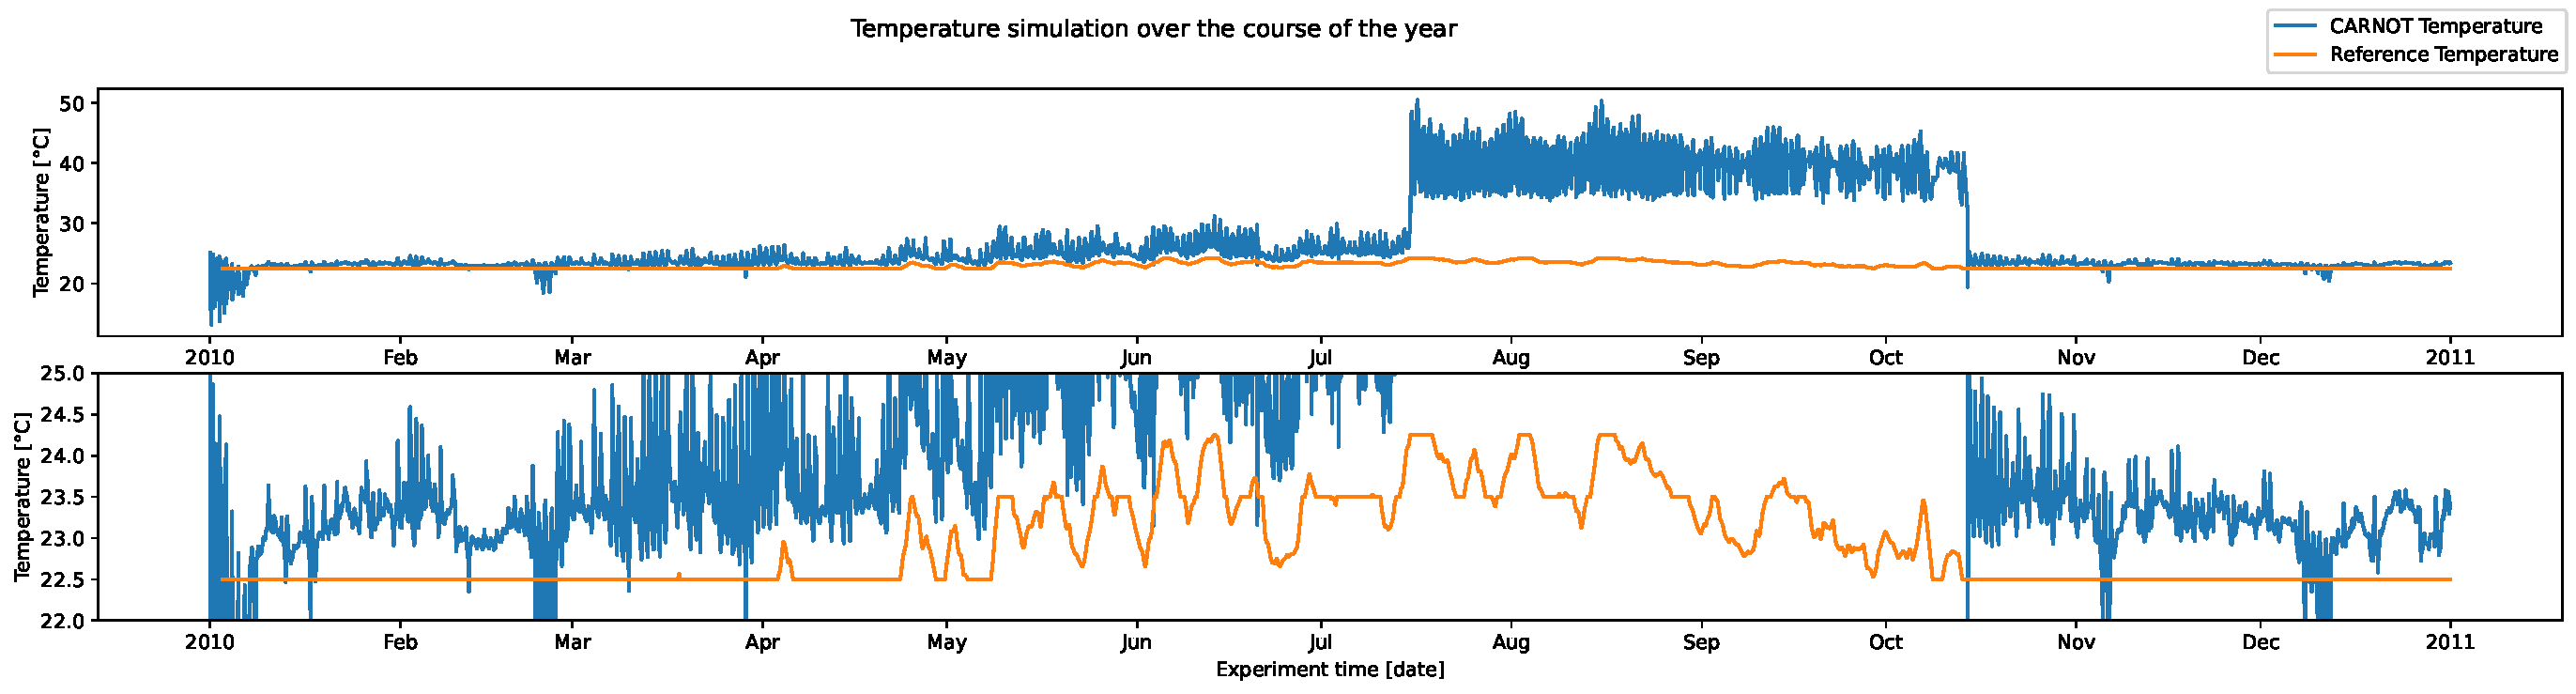
\includegraphics[width =
    \textwidth]{Plots/4_GP_480pts_12_averageYear_fullyear.pdf}
    \caption{GP full year simulation}
    \label{fig:GP_fullyear_simulation}
\end{figure}

This very large difference in performance could be explained by the change in
weather during the year. The winter months of the beginning and end of the year
exhibit similar performance. The spring months already make the controller less
stable than at the start of the year, while the drastic temperature changes in
the summer make the controller completely unstable.

Figure~\ref{fig:GP_fullyear_abserr} presents the absolute error measured at each
step of the simulation over the course of the year. We can note a mean absolute
error of 1.33 $\degree$C, with the largest deviations occurring in late summer
where the absolute error can reach extreme values, and the `best' performance
occurring during the winter months. 

\begin{figure}[ht]
    \centering
    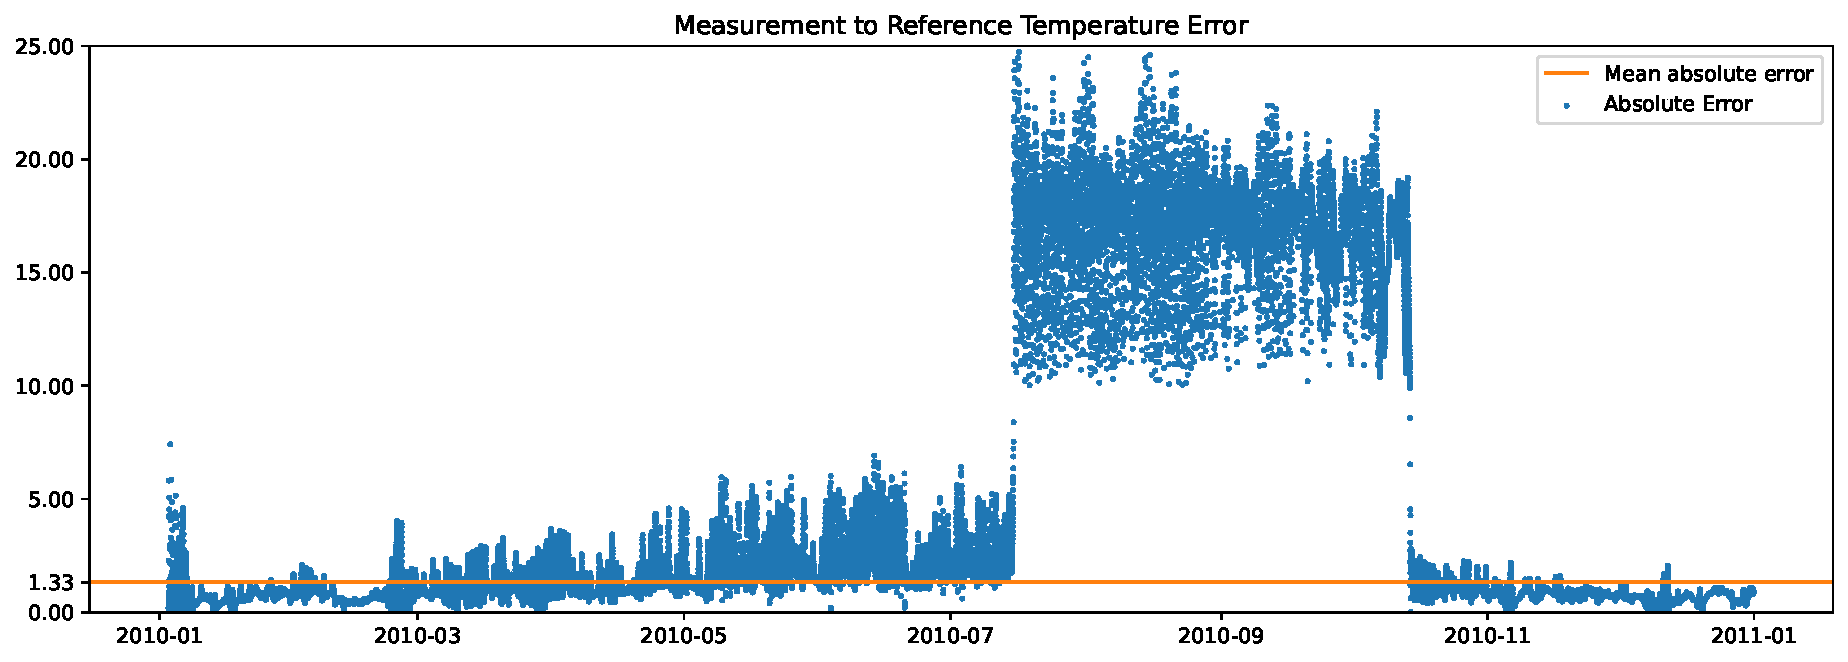
\includegraphics[width =
    \textwidth]{Plots/4_GP_480pts_12_averageYear_abserr.pdf}
    \caption{GP full year absolute error}
    \label{fig:GP_fullyear_abserr}
\end{figure}

Figure~\ref{fig:GP_first_model_performance} analyzes the 20-step ahead
simulation performance of the identified model over the course of the year. At
experimental step 250, the controller is still gathering data. It is therefore
expected that the identified model will be capable of reproducing this data. At
step 500, 20 steps after identification, the model correctly steers the internal
temperature towards the reference temperature. On the flip side, already at
experimental steps 750 and 1000, only 9 days into the simulation, the model is
unable to properly simulate the behaviour of the plant, with the maximum
difference at the end of the simulation reaching 0.75 $\degree$C and 1.5
$\degree$C respectively.

\begin{figure}[ht]
    \centering
    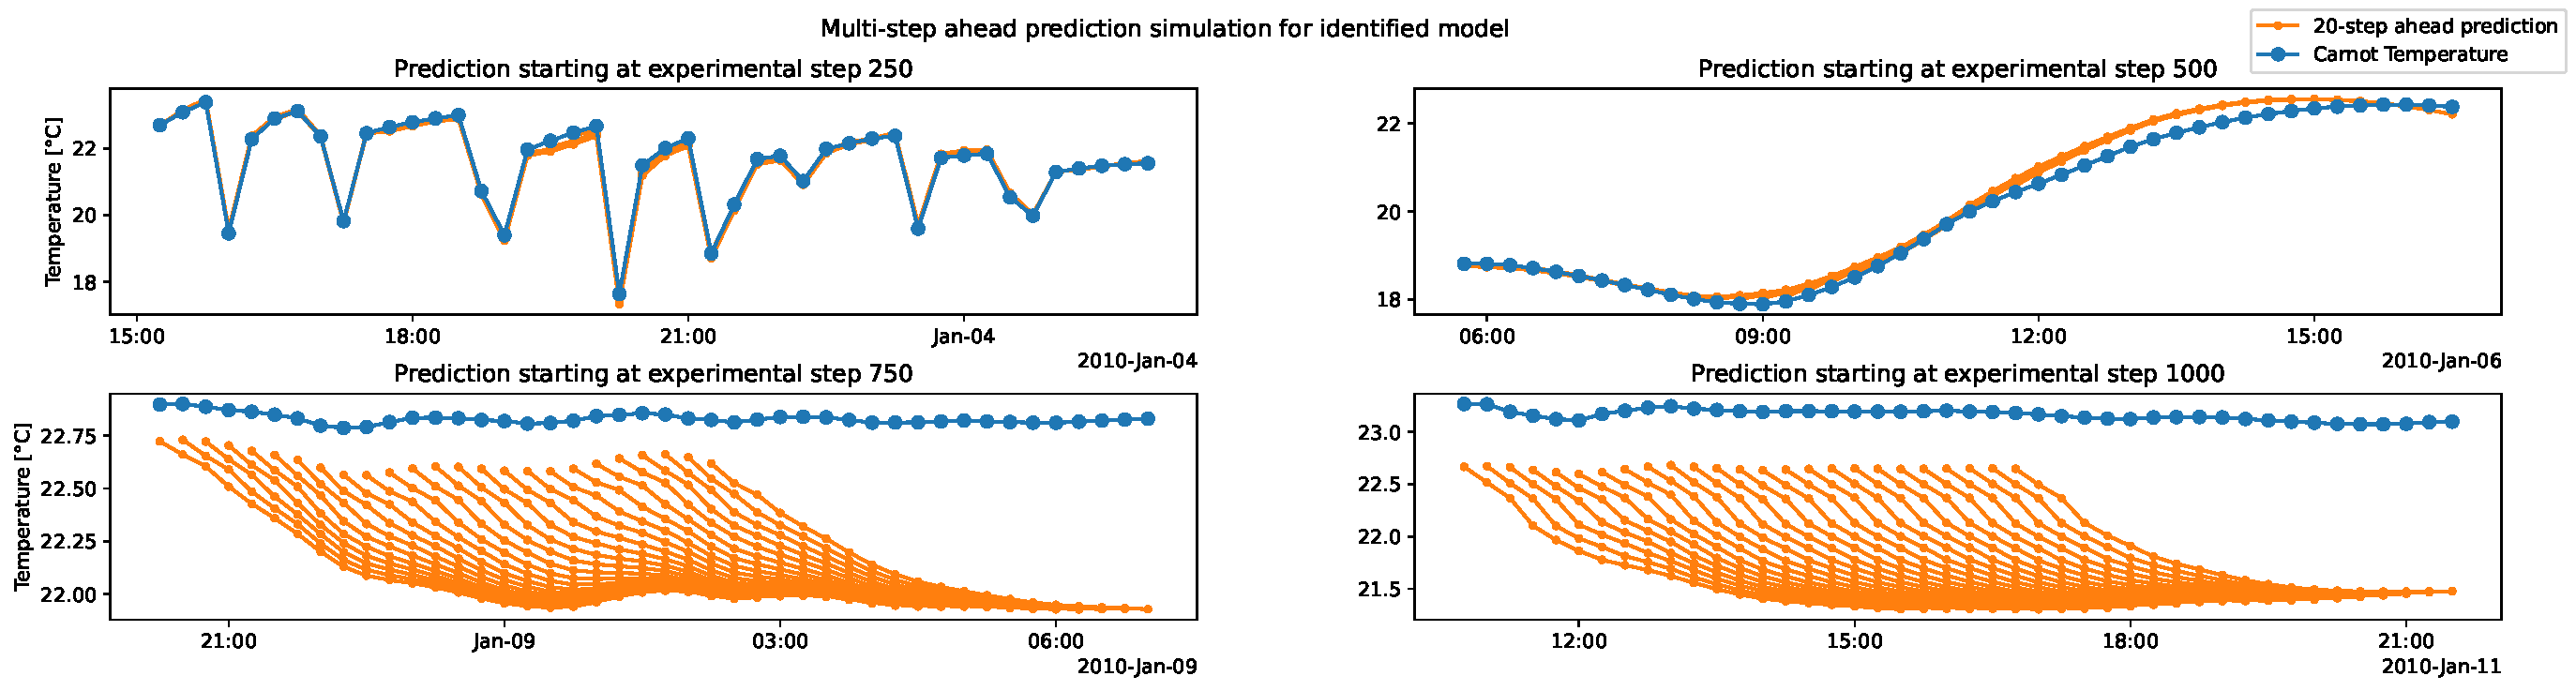
\includegraphics[width =
    \textwidth]{Plots/4_GP_480pts_12_averageYear_first_model_performance.pdf}
    \caption{GP model performance}
    \label{fig:GP_first_model_performance}
\end{figure}

This large difference of performance could be explained by the change in outside
weather (solar irradiance and outside temperature --- the exogenous inputs) from
the one present during the training phase. It can be seen in
Figure~\ref{fig:Dataset_outside_temperature} that already at 500 points in the
simulation both the GHI and the Outside Temperature are outside of the training
ranges, with the latter exhibiting a much larger variation. 


\begin{figure}[ht]
    \centering
    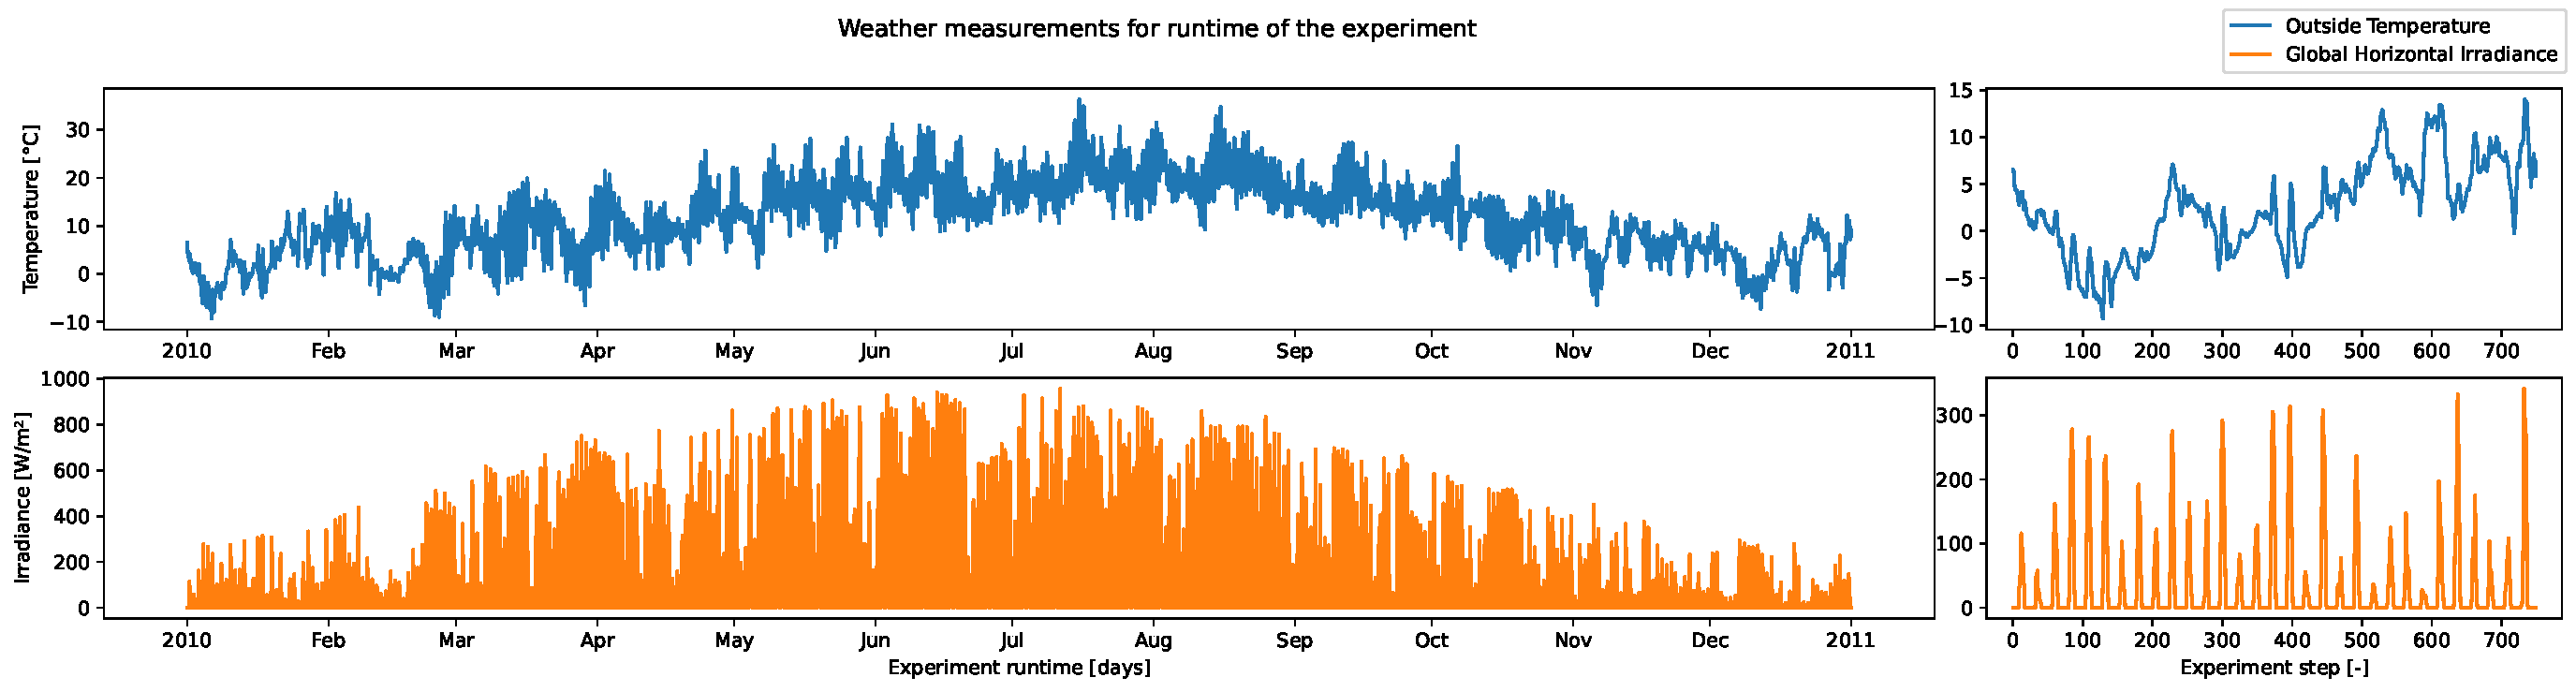
\includegraphics[width =
    \textwidth]{Plots/Exogenous_inputs_fullyear.pdf}
    \caption{Exogenous inputs for the simulation}
    \label{fig:Dataset_outside_temperature}
\end{figure}

Finally, it is possible to conclude that this approach does not perform well due
to several causes:

\begin{itemize}
    \item The size of the training dataset is limited by the computation budget
    \item The model does not extrapolate correctly the information on
        disturbances
    \item The model stays fixed for the duration of the year, being unable to
        adapt to new weather conditions.
\end{itemize}

These problems could be solved in several ways, such as periodically
re-identifying the model to fit the current weather pattern. This approach would
be quite cumbersome due to repeated need of disturbing the model in order to
sufficiently excite it. Another approach would be to keep the whole historical
dataset of measurements, which quickly renders the problem intractable. More
complex solutions, such as keeping a fixed-size data dictionary whose points are
deleted when they no longer help the predictions and new points are added as
they are deemed useful or compiling the training dataset with multiple
experiments in different weather conditions could dramatically improve model
performance, but are more complex in implementation.


\subsection{Sparse and Variational Gaussian Process}\label{sec:SVGP_results}

The \acrlong{svgp} models are setup in a similar way as described before. The
model is first identified using 5 days worth of experimental data collected
using a \acrshort{pi} controller and a random disturbance signal. The difference
lies in the fact than the \acrshort{svgp} model gets re-identified every night
at midnight using the newly accumulated data from closed-loop operation.

The results of this setup are presented in
Figure~\ref{fig:SVGP_fullyear_simulation}. It can already be seen that this
setup performs much better than the initial one. The only large deviations from
the reference temperature are due to cold weather, when the \acrshort{hvac}'s
limited heat capacity is unable to maintain the proper temperature.
Additionnaly, the \acrshort{svgp} controller takes around 250 - 300ms of
computation time for each simulation time, decreasing the computational cost of
the original \acrshort{gp} by a factor of six.



\begin{figure}[ht]
    \centering
    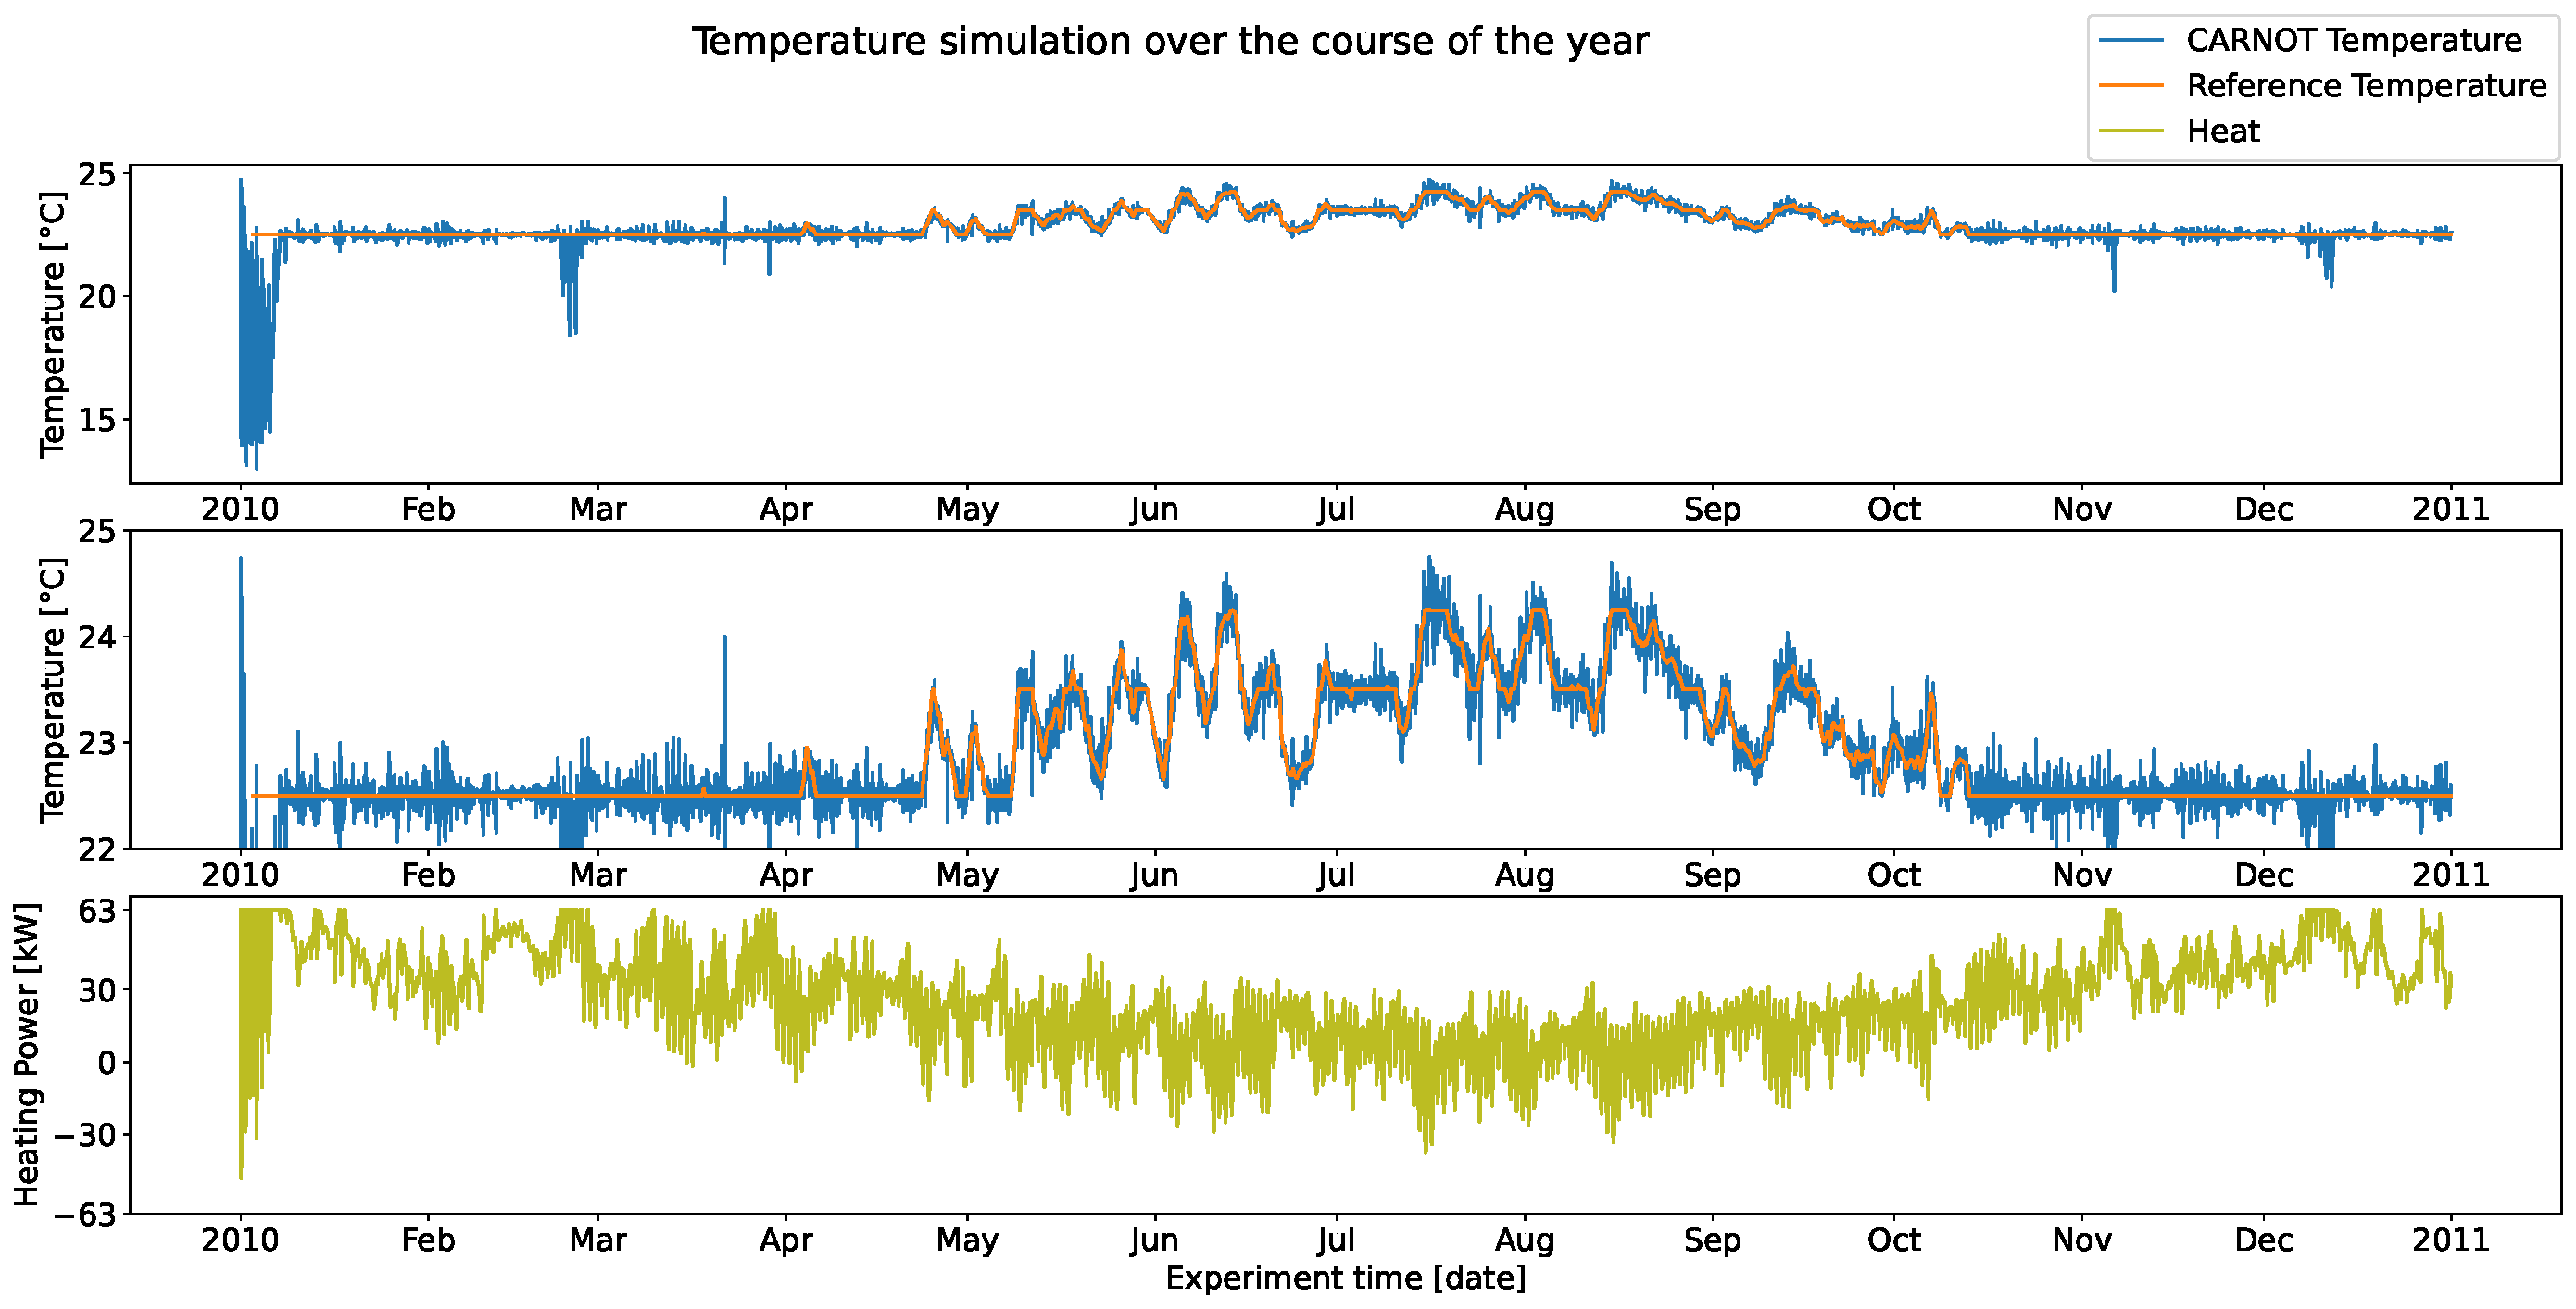
\includegraphics[width =
    \textwidth]{Plots/1_SVGP_480pts_inf_window_12_averageYear_fullyear.pdf}
    \caption{SVGP full year simulation}
    \label{fig:SVGP_fullyear_simulation}
\end{figure}

\clearpage

Comparing the absolute error of the measured vs reference temperature for the
duration of the experiment (cf. Figure~\ref{fig:SVGP_fullyear_abserr}) with the
one of the original experiment, the average absolute error is reduced from 1.33
$\degree$C to only 0.05 $\degree$C, with the majority of the values being lower
than 0.4 $\degree$ C. 

\begin{figure}[ht]
    \centering
    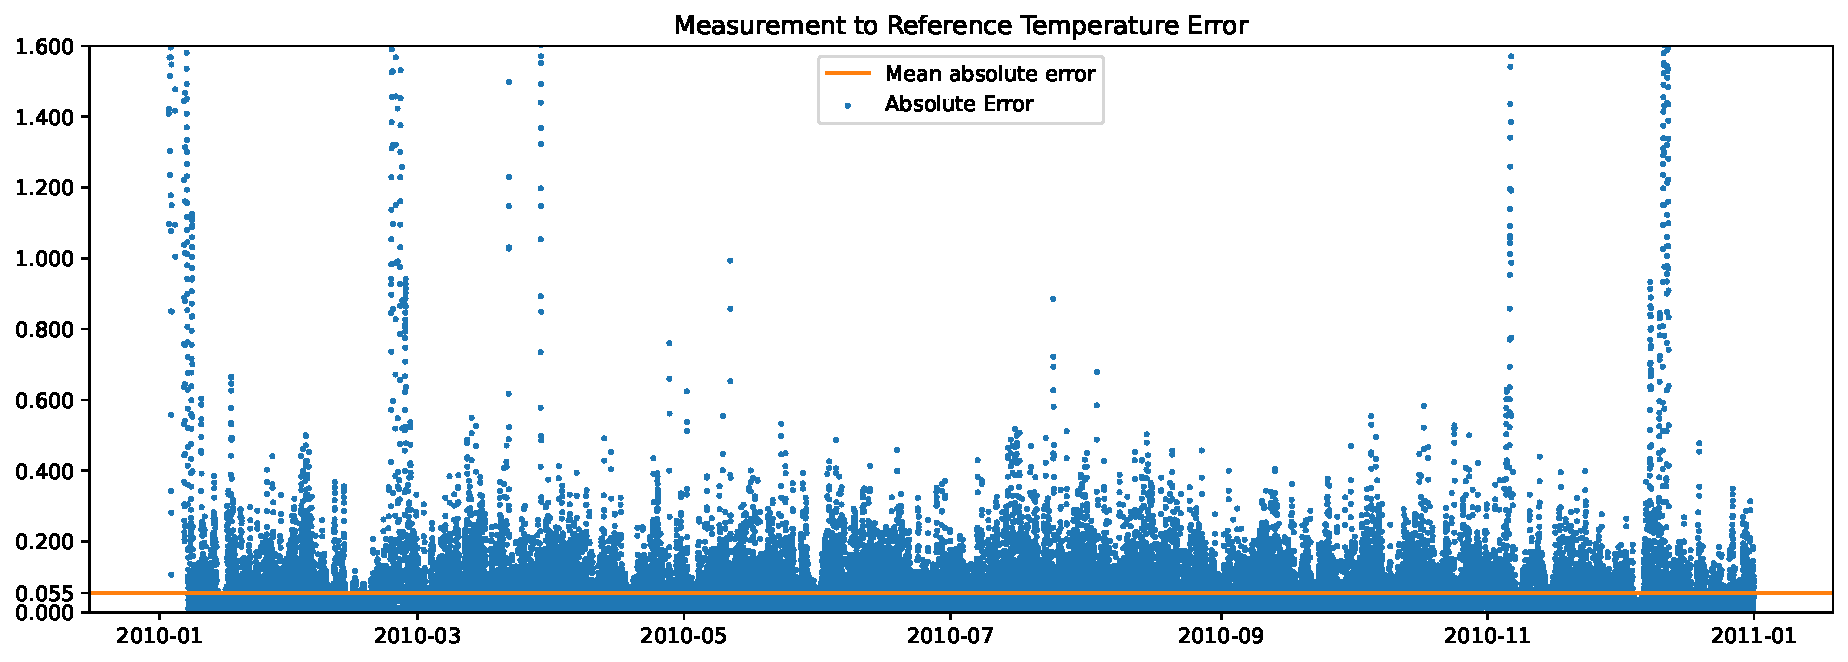
\includegraphics[width =
    \textwidth]{Plots/1_SVGP_480pts_inf_window_12_averageYear_abserr.pdf}
    \caption{SVGP full year absolute error}
    \label{fig:SVGP_fullyear_abserr}
\end{figure}

Figures~\ref{fig:SVGP_first_model_performance},
~\ref{fig:SVGP_later_model_performance}
and~\ref{fig:SVGP_last_model_performance} show the 20-step simulation performance of three
different models, identified at three different stages of the experiment. They
have all been set to simulate 25 consecutive experimental steps starting at
steps 250, 500, 10750 and 11000 respectively.

The initial model (cf. Figure~\ref{fig:SVGP_first_model_performance}),
identified after the first five days has the worst performance. It is unable to
correctly simulate even the learning dataset. This behaviour is similar to that
discovered in Figure~\ref{fig:SVGP_multistep_validation}
(cf. Section~\ref{sec:validation_hyperparameters}), where the \acrshort{svgp}
model performed worse than the equivalent \acrshort{gp} trained on the same
dataset. It also performs worse than the initial \acrshort{gp} model in the rest
of the simulations, being unable to correctly predict the heating to reference
at step 500, and having maximum errors of around 10 $\degree$C for the simulations
starting at 107500 and 11000 points.

\begin{figure}[ht]
    \centering
    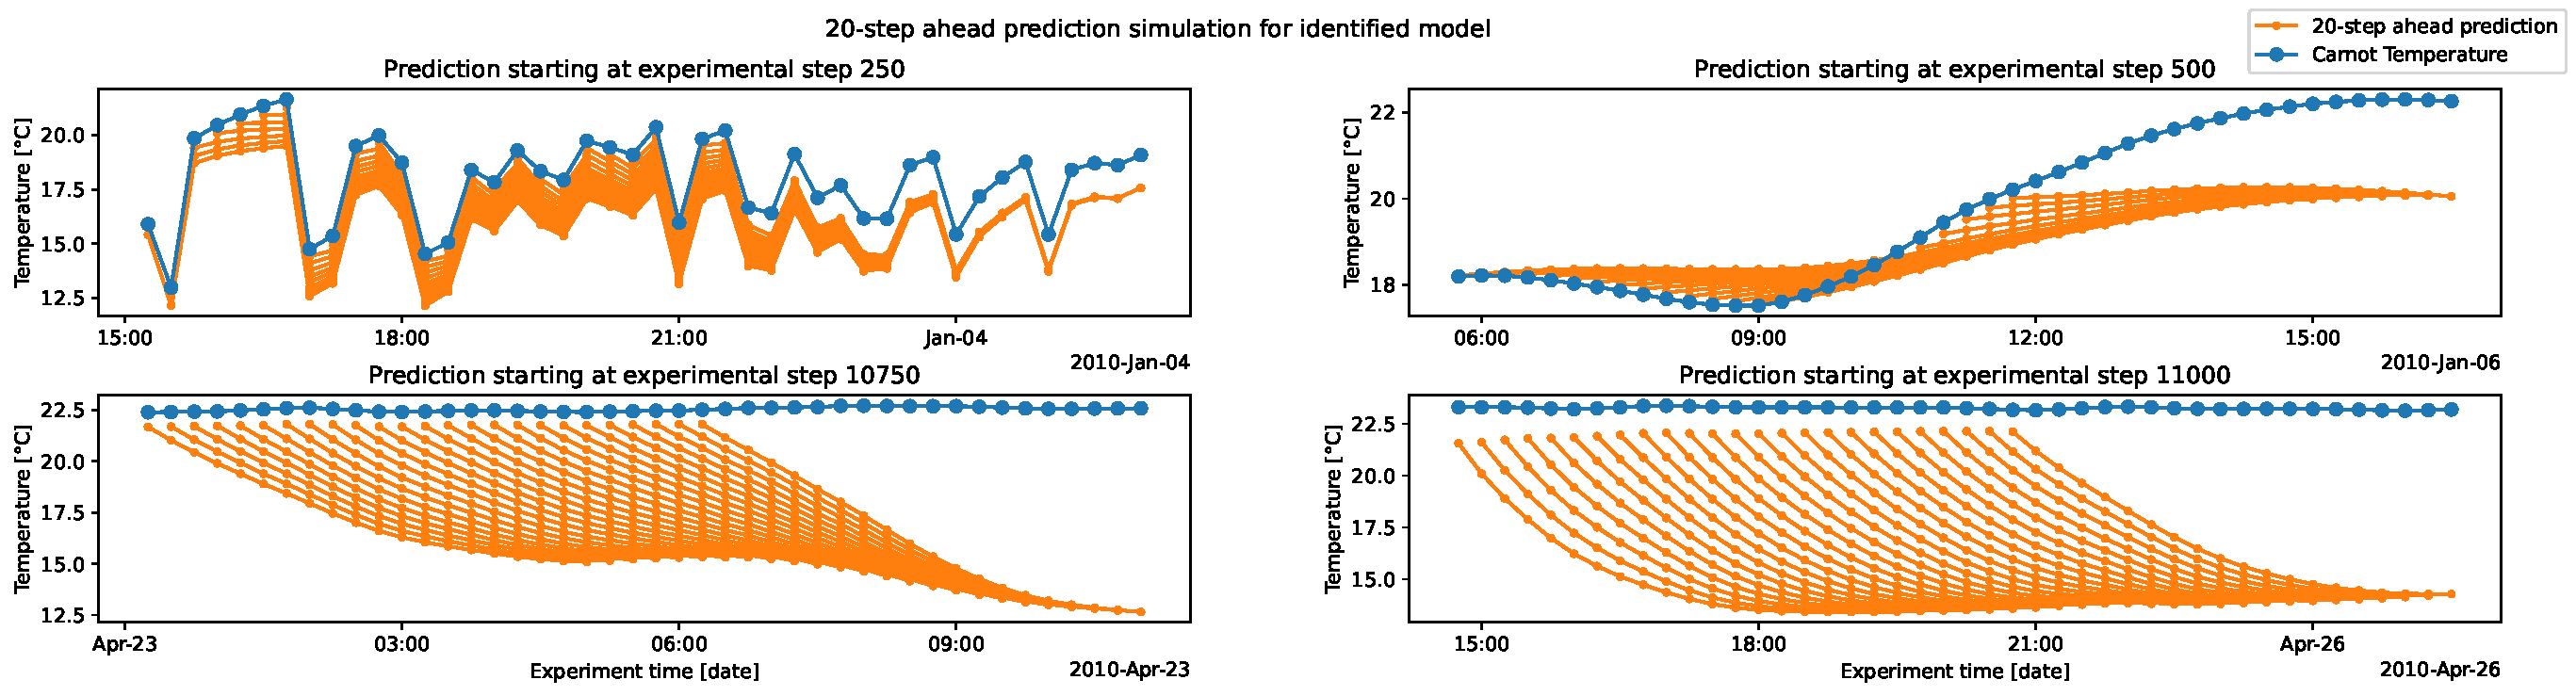
\includegraphics[width =
    \textwidth]{Plots/1_SVGP_480pts_inf_window_12_averageYear_first_model_performance.pdf}
    \caption{SVGP first model performance}
    \label{fig:SVGP_first_model_performance}
\end{figure}

\clearpage

Figure~\ref{fig:SVGP_later_model_performance} shows the performance of the 100th
trained model (i.e the model trained on April 15). This model performs much
better in all simulations. It is able to correctly simulate the 20-step
behaviour of the plant over all the experimental steps in the first two cases.
It still has a noticeable error when predicting the behaviour of the plant on
new data (i.e. simulations starting at steps 10750 and 11000), but it is much
less than before. This gives a hint at the fact that the \acrshort{svgp} model's
performance improves throughout the year, but it does require much more data
than the classical \acrshort{gp} model to capture the building dynamics.

\begin{figure}[ht]
    \centering
    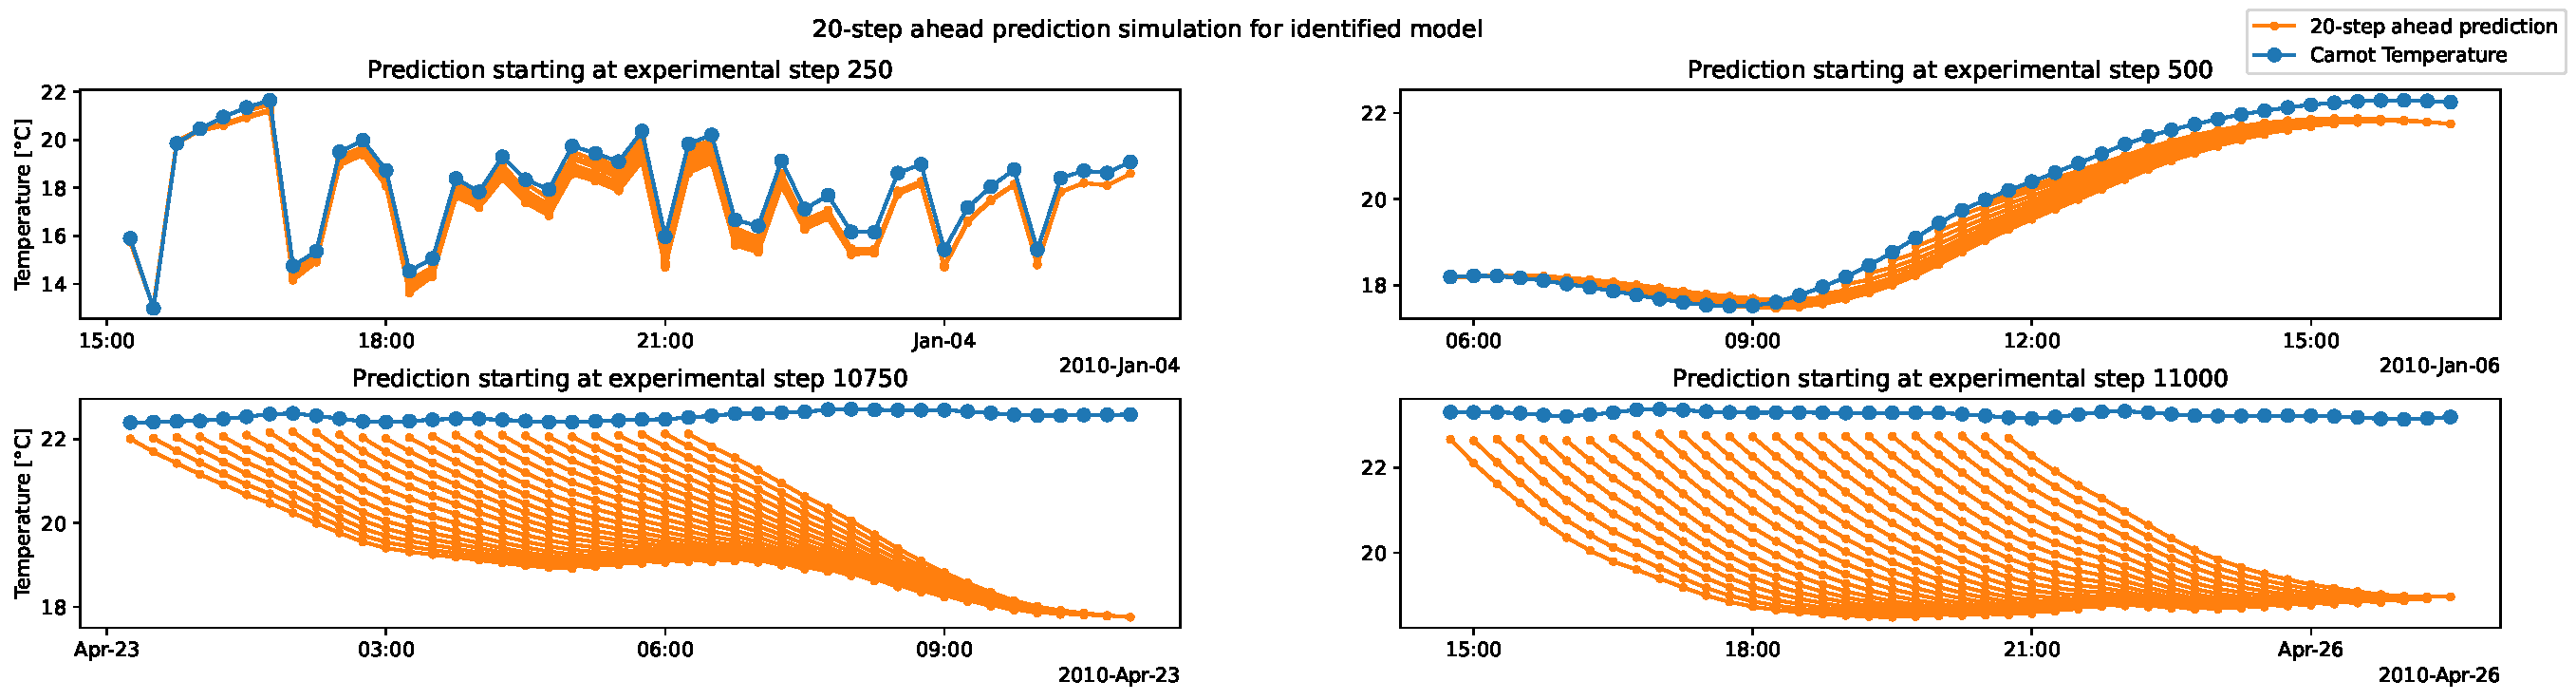
\includegraphics[width =
    \textwidth]{Plots/1_SVGP_480pts_inf_window_12_averageYear_later_model_performance.pdf}
    \caption{SVGP later model performance}
    \label{fig:SVGP_later_model_performance}
\end{figure}

The last model is trained on the whole-year dataset.
Figure~\ref{fig:SVGP_last_model_performance} shows its performance for the same
situation described before. The model is able to predict the plant's behaviour
at steps 250 and 500 even better than before, as well as predict the behaviour
at steps 10750 and 11000 with maximum error of 0.6 $\degree$C and 0.1 $\degree$C
respectively.

\begin{figure}[ht]
    \centering
    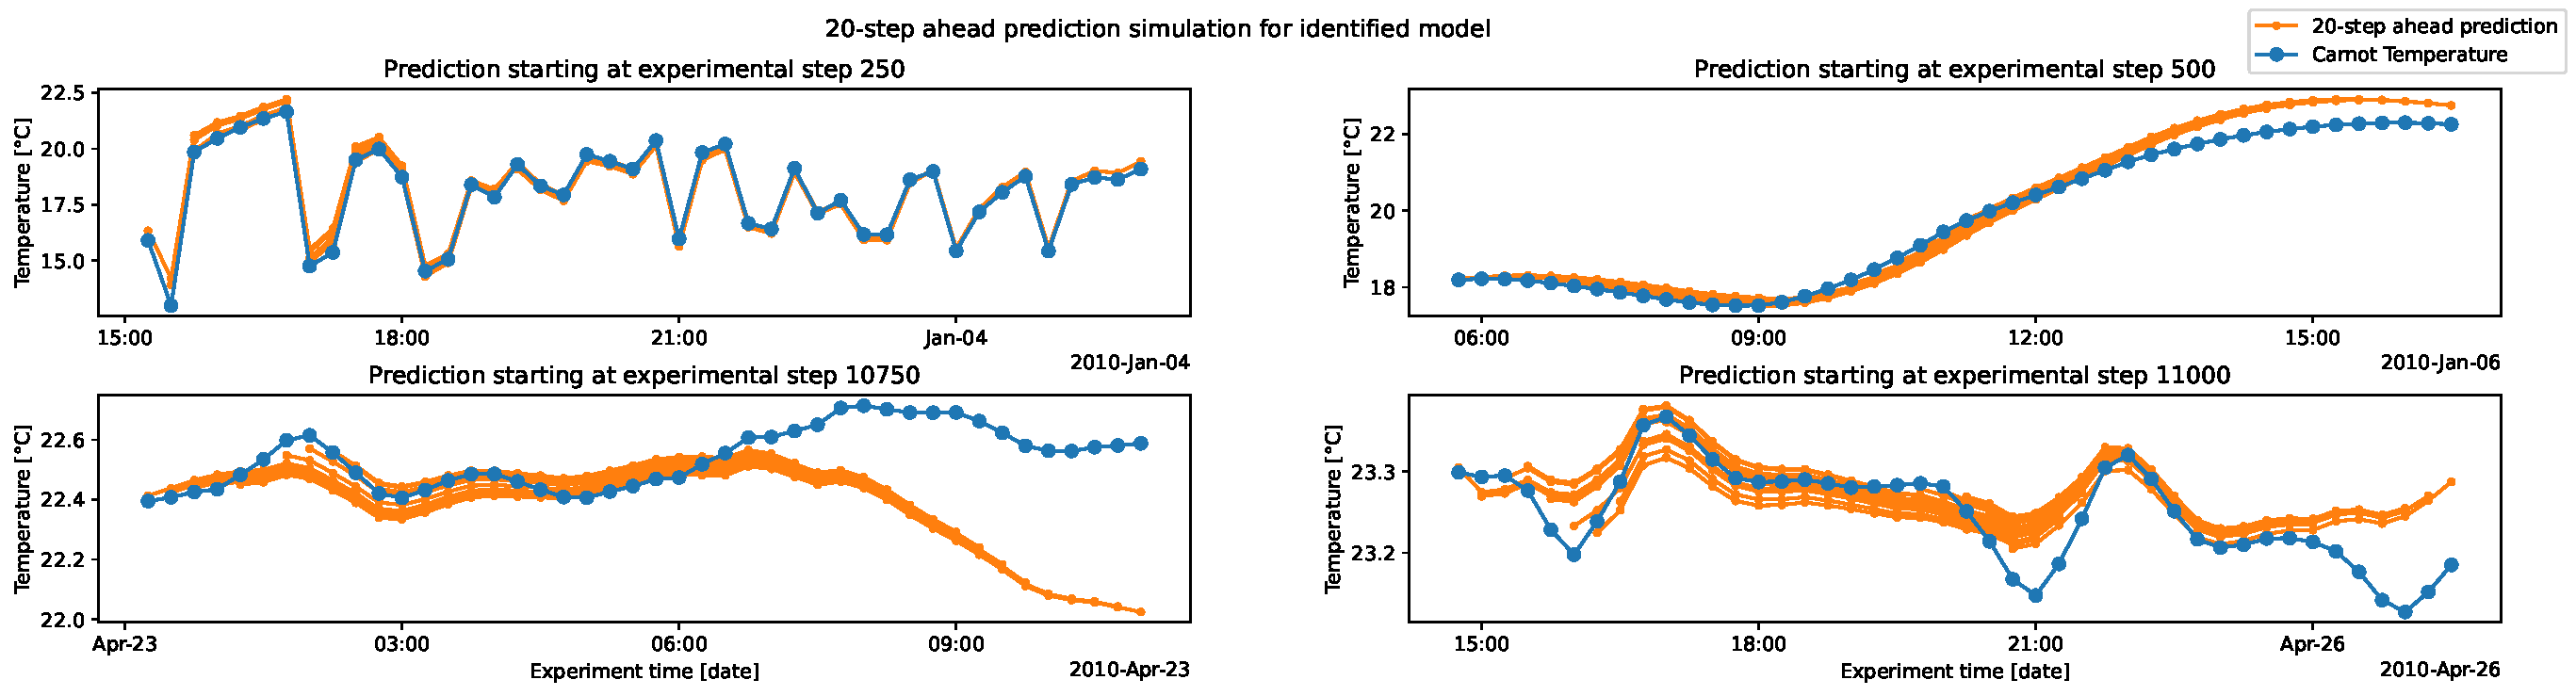
\includegraphics[width =
    \textwidth]{Plots/1_SVGP_480pts_inf_window_12_averageYear_last_model_performance.pdf}
    \caption{SVGP last model performance}
    \label{fig:SVGP_last_model_performance}
\end{figure}

The analysis of the model evolution as more data gets gathered already gives
very good insight into the strengths and weaknesses of this approach. The
initial model is unable to correctly extrapolate the plant's behaviour in new
regions of the state space. Also, given the same amount of data, the
\acrshort{svgp} model is able to capture less information about the plant
dynamics than the equivalent \acrshort{gp} model. On the flip side, re-training
the model every day with new information is able to mitigate this by adding the
data in new regions as it gets discovered while being able to maintain constant
training and evaluation cost.

A more in depth analysis of the evolution of the \acrshort{svgp} hyperparameters
over the duration of the experiment is presented in
Section~\ref{sec:lengthscales_results}.

A few questions arise naturally after investigating the performance of this
control scheme: 

\begin{itemize}
    \item If the model is able to correctly understand data gathered in
        closed-loop operation, will the performance deteriorate drastically if
        the first model is trained on less data?
    \item How much information can the model extract from closed-loop operation?
        Would a model trained on a window of only the last five days of 
        closed-loop operation data be able to perform correctly?
\end{itemize}

These questions will be further analysed in the Sections~\ref{sec:svgp_96pts}
and~\ref{sec:svgp_window} respectively.

\clearpage

\subsubsection{Lengthscales}\label{sec:lengthscales_results}

Figure~\ref{fig:SVGP_evol_importance} provides a deeper insight into the
evolution of the relative importance of the \acrshort{svgp} regressors over the
course of the full-year simulation\footnotemark. A few remarks are immediate:
the importance of most hyperparameters changes drastically the first few
iterations, until reaching a more steady change pace, until around the month of
July where most of the hyperparameters settle for the rest of the simulation.
This behaviour could be explained by the model learning new regions of the state
space (i.e the span of the \acrshort{ghi} and Outside Temperatures) over the
first months as these values change, and remaining more constant once it has
already gathered information on these different operating points.

\footnotetext{The evolution of the \textit{hyperparameters} is provided for
reference in Annex~\ref{anx:hyperparams_evol}.}

\begin{figure}[ht]
    \centering
    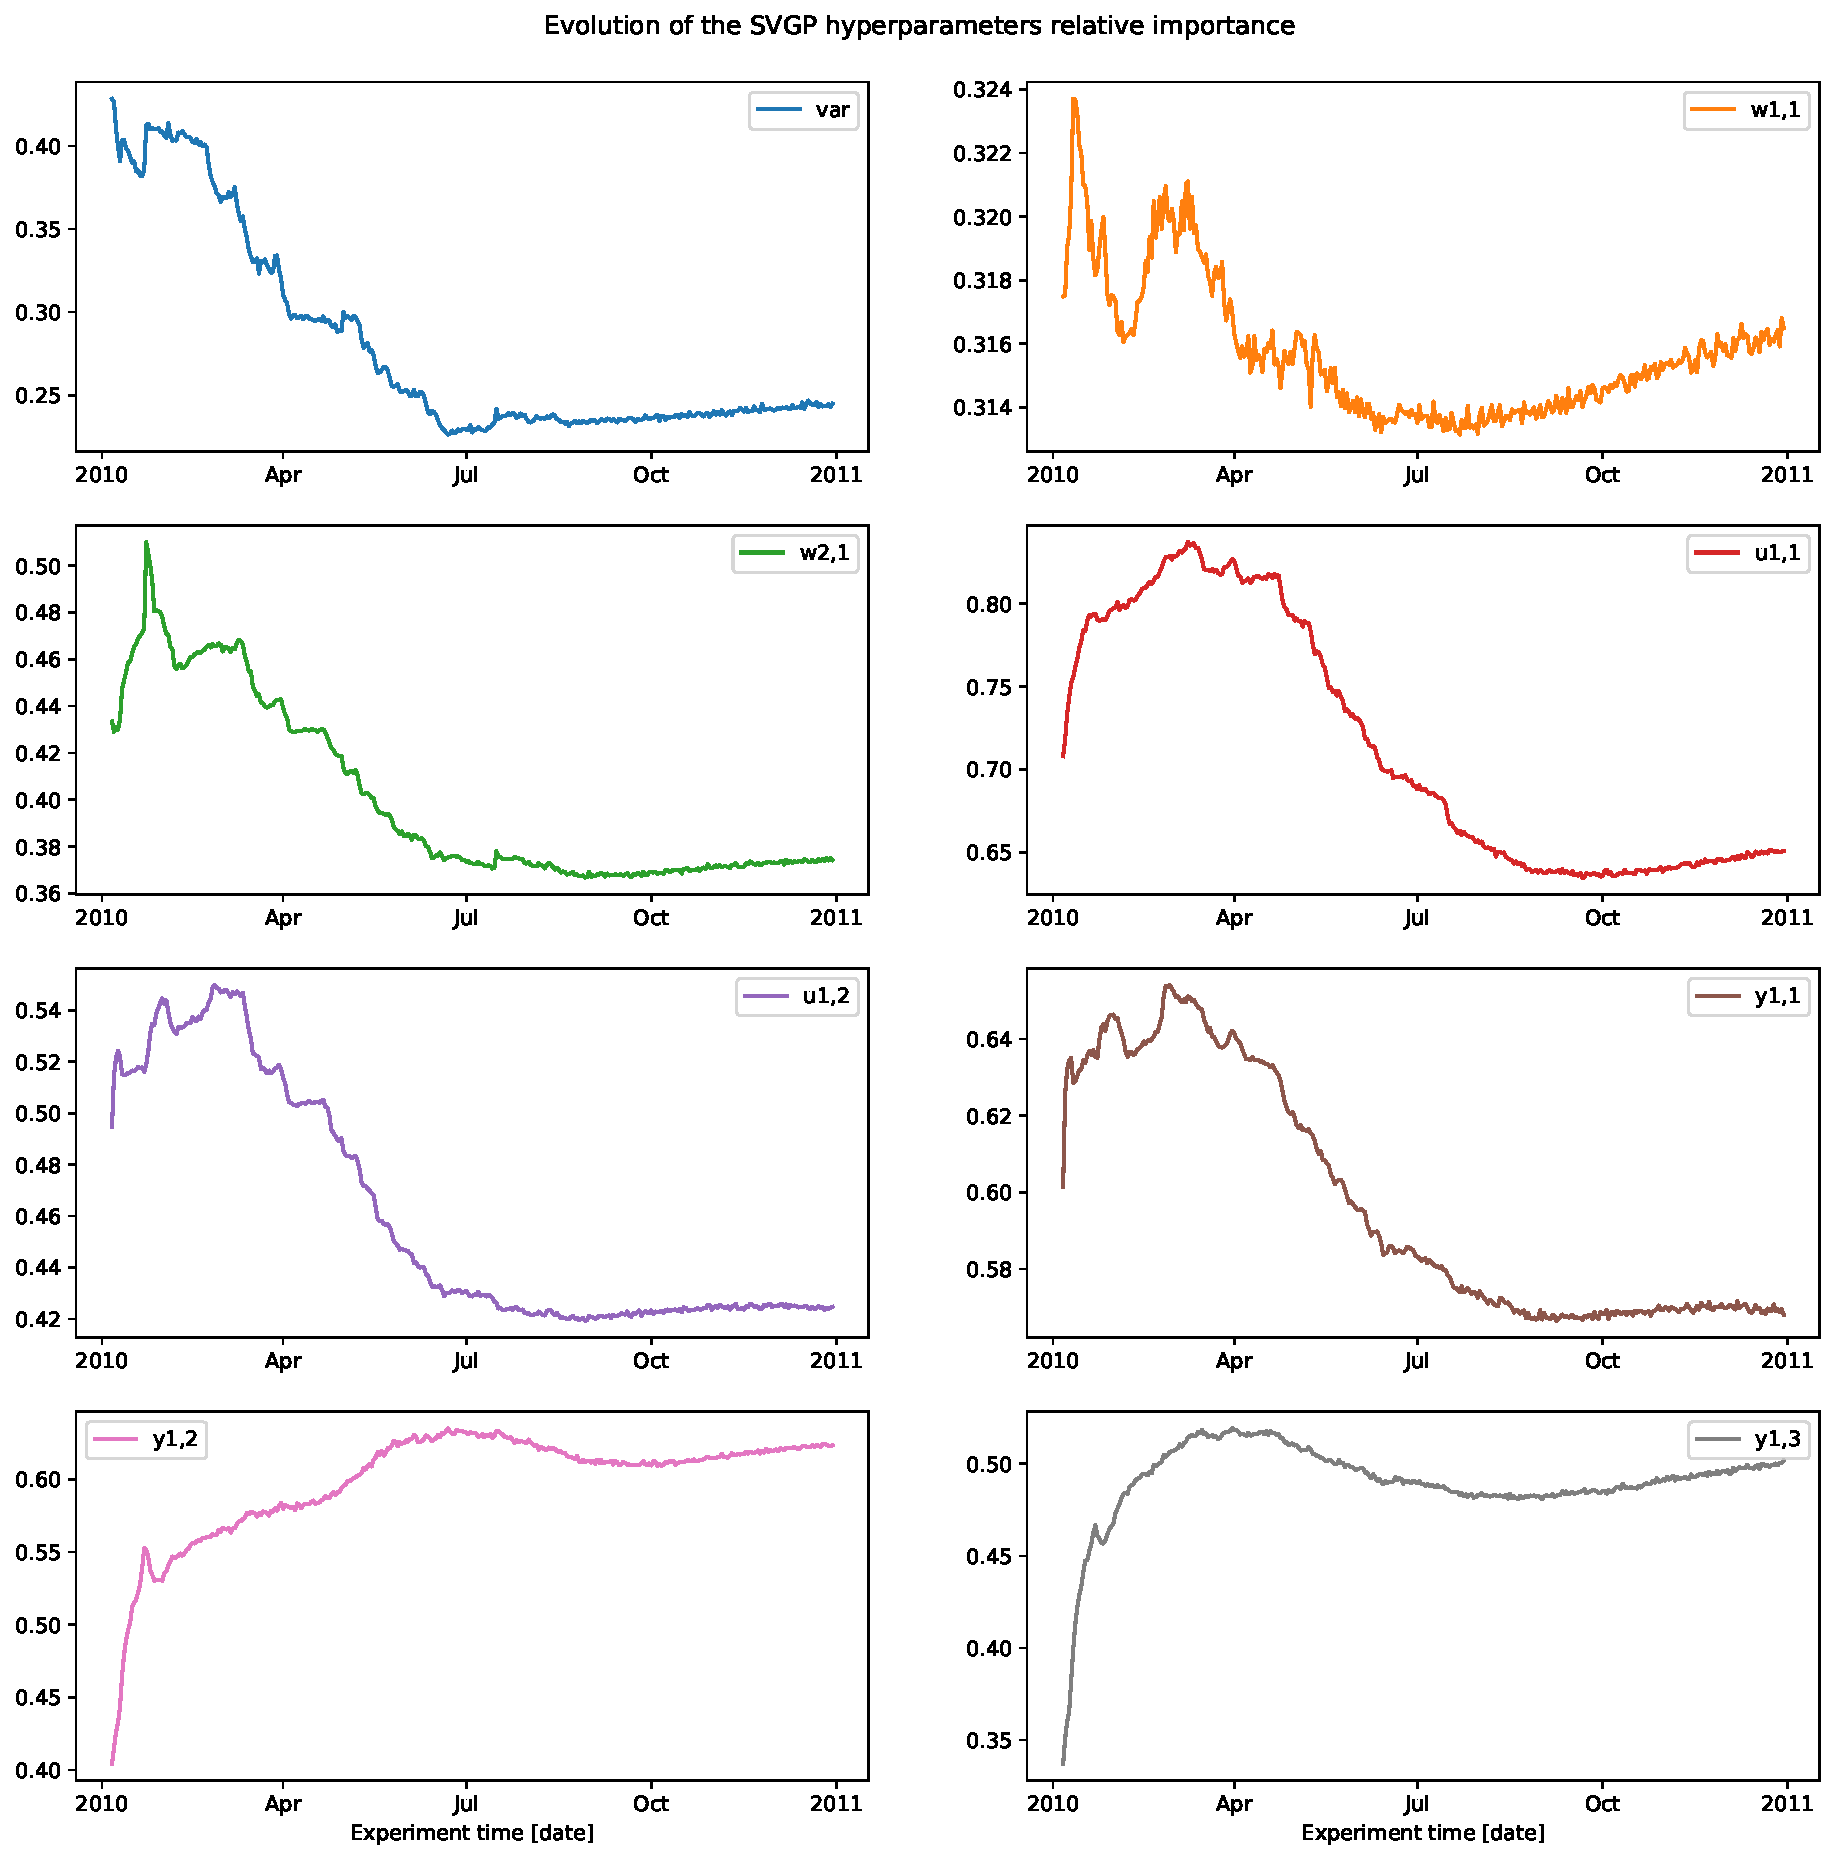
\includegraphics[width =
    \textwidth]{Plots/1_SVGP_480pts_inf_window_12_averageYear_evol_importance.pdf}
    \caption{Evolution of SVGP model parameters}
    \label{fig:SVGP_evol_importance}
\end{figure}

As seen in Figure~\ref{fig:SVGP_evol_importance}, the variance of the
\acrshort{se} kernel steadily decreases, until reaching a plateau, which
signifies the increase in confidence of the model. The hyperparameters
corresponding to the exogenous inputs --- $w1,1$ and $w1,2$ --- become generally
less important for future predictions over the course of the year, with the
importance of $w1,1$, the \acrlong{ghi}, climbing back up over the last, colder
months. This might be due to the fact that during the colder months, the
\acrshort{ghi} is the only way for the exogenous inputs to \textit{provide}
additional heat to the system.

A similar trend can be observed for the evolution of the input's
hyperparameters, with the exception that the first lag of the controlled input
($u1,1$) remains the most important over the course of the year.

For the lags of the measured output it can be seen that, over the course of the
year, the importance of the first lag decreases, while that of the second and
third lag increase --- until all three reach relatively similar values.

Another interesting comparison is provided by looking at the possible values of
the \acrshort{se} kernel components. Since all the values are normalized within
the -1 to 1 range, it is unlikely that any two points will be a distance higher
than 2 apart. It is possible then to plot the values of the kernel terms due to
each regressor as a function of their distance. This is done in
Figure~\ref{fig:SVGP_first_covariance} for the first identified model and in
Figure~\ref{fig:SVGP_last_covariance} for the last. It is clear that in both
cases the kernel terms behave mostly linearly, with the exception of two points
being close to each other, when the correlation remains stronger before it
starts diminishing.

\begin{figure}[ht]
    \centering
    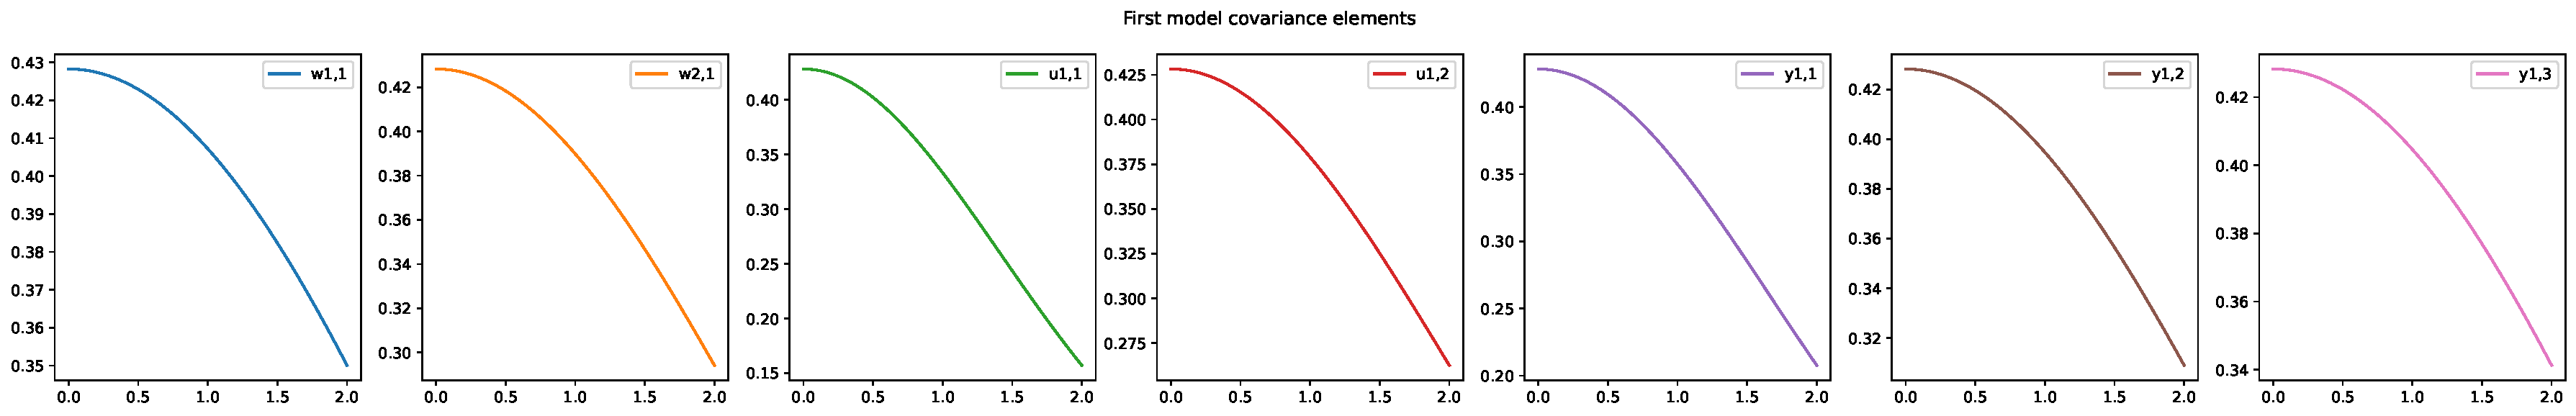
\includegraphics[width =
    \textwidth]{Plots/1_SVGP_480pts_inf_window_12_averageYear_first_covariance.pdf}
    \caption{SVGP model first covariance parameters}
    \label{fig:SVGP_first_covariance}
\end{figure}

As for the last model, it can be noted that only the scale of the kernel terms
changes, with their shape remaining consistent with the first identified model.
This means that the model does not get much more complex as the data is
gathered, but instead the same general structure is kept, with further
refinements being done as data is added to the system.

\clearpage

\begin{figure}[ht]
    \centering
    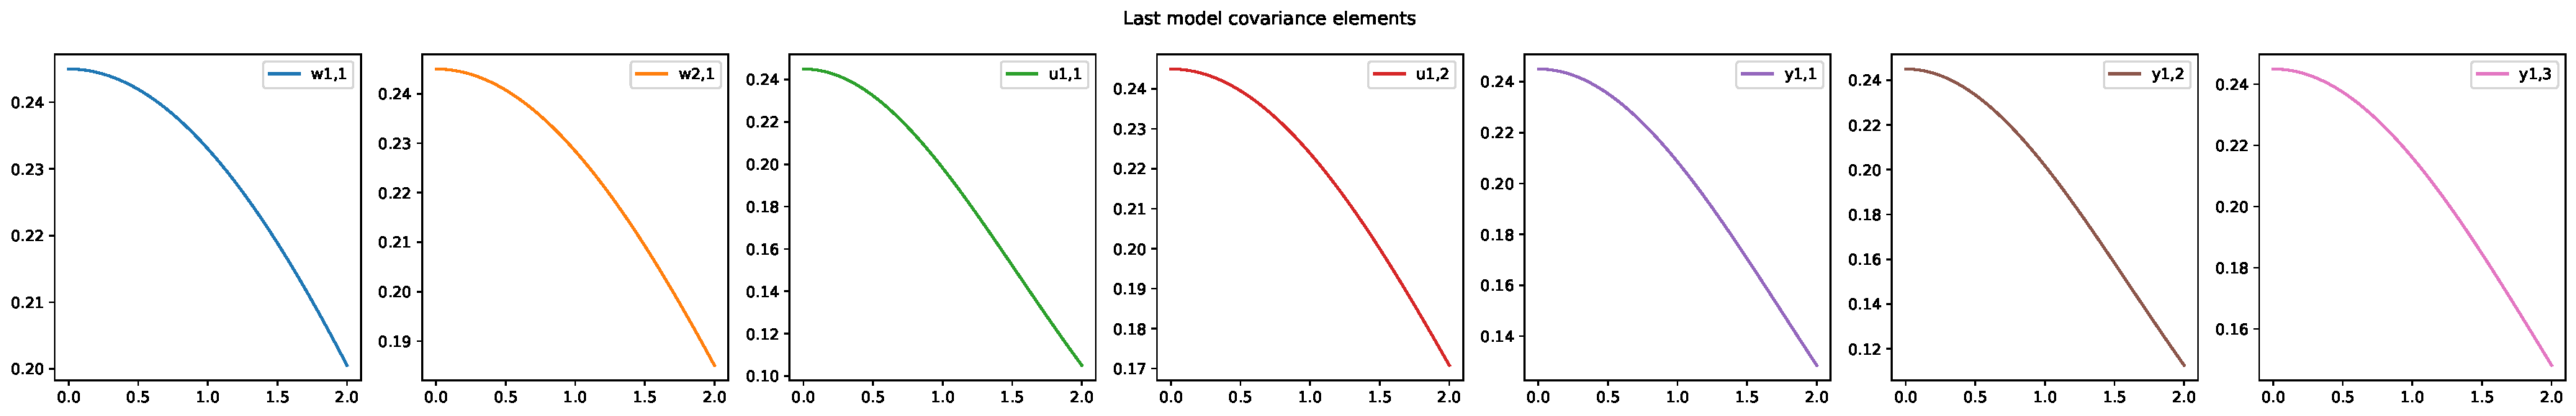
\includegraphics[width =
    \textwidth]{Plots/1_SVGP_480pts_inf_window_12_averageYear_last_covariance.pdf}
    \caption{SVGP model last covariance parameters}
    \label{fig:SVGP_last_covariance}
\end{figure}

One question that could be addressed given these mostly linear kernel terms is
how well would an \acrshort{svgp} model perform with a linear kernel.
Intuition would hint that it should still be able to track the reference
temperature, albeit not as precisely due to the correlation that diminishes much
slower when the two points are closer together in the \acrshort{se} kernel. This
will be further investigated in Section~\ref{sec:svgp_linear}.

\clearpage

\subsection{SVGP with one day of starting data}\label{sec:svgp_96pts}

As previously discussed in Section~\ref{sec:SVGP_results}, the \acrshort{svgp}
model is able to properly adapt given new information, overtime refining its
understanding of the plant's dynamics.

Analyzing the results of a simulation done on only one day's worth of initial
simulation data (cf. Figures~\ref{fig:SVGP_96pts_fullyear_simulation}
and~\ref{fig:SVGP_96pts_abserr}) it is very notable that the model performs
almost identically to the one identified in the previous sections. This
highlights one of the practical benefits of the \acrshort{svgp} implementations
compared to the classical \acrlong{gp} -- it is possible to start with a rougher
controller trained on less data and refine it over time, reducing the need for
cumbersome and potentially costly initial experiments for gathering data.

\begin{figure}[ht]
    \centering
    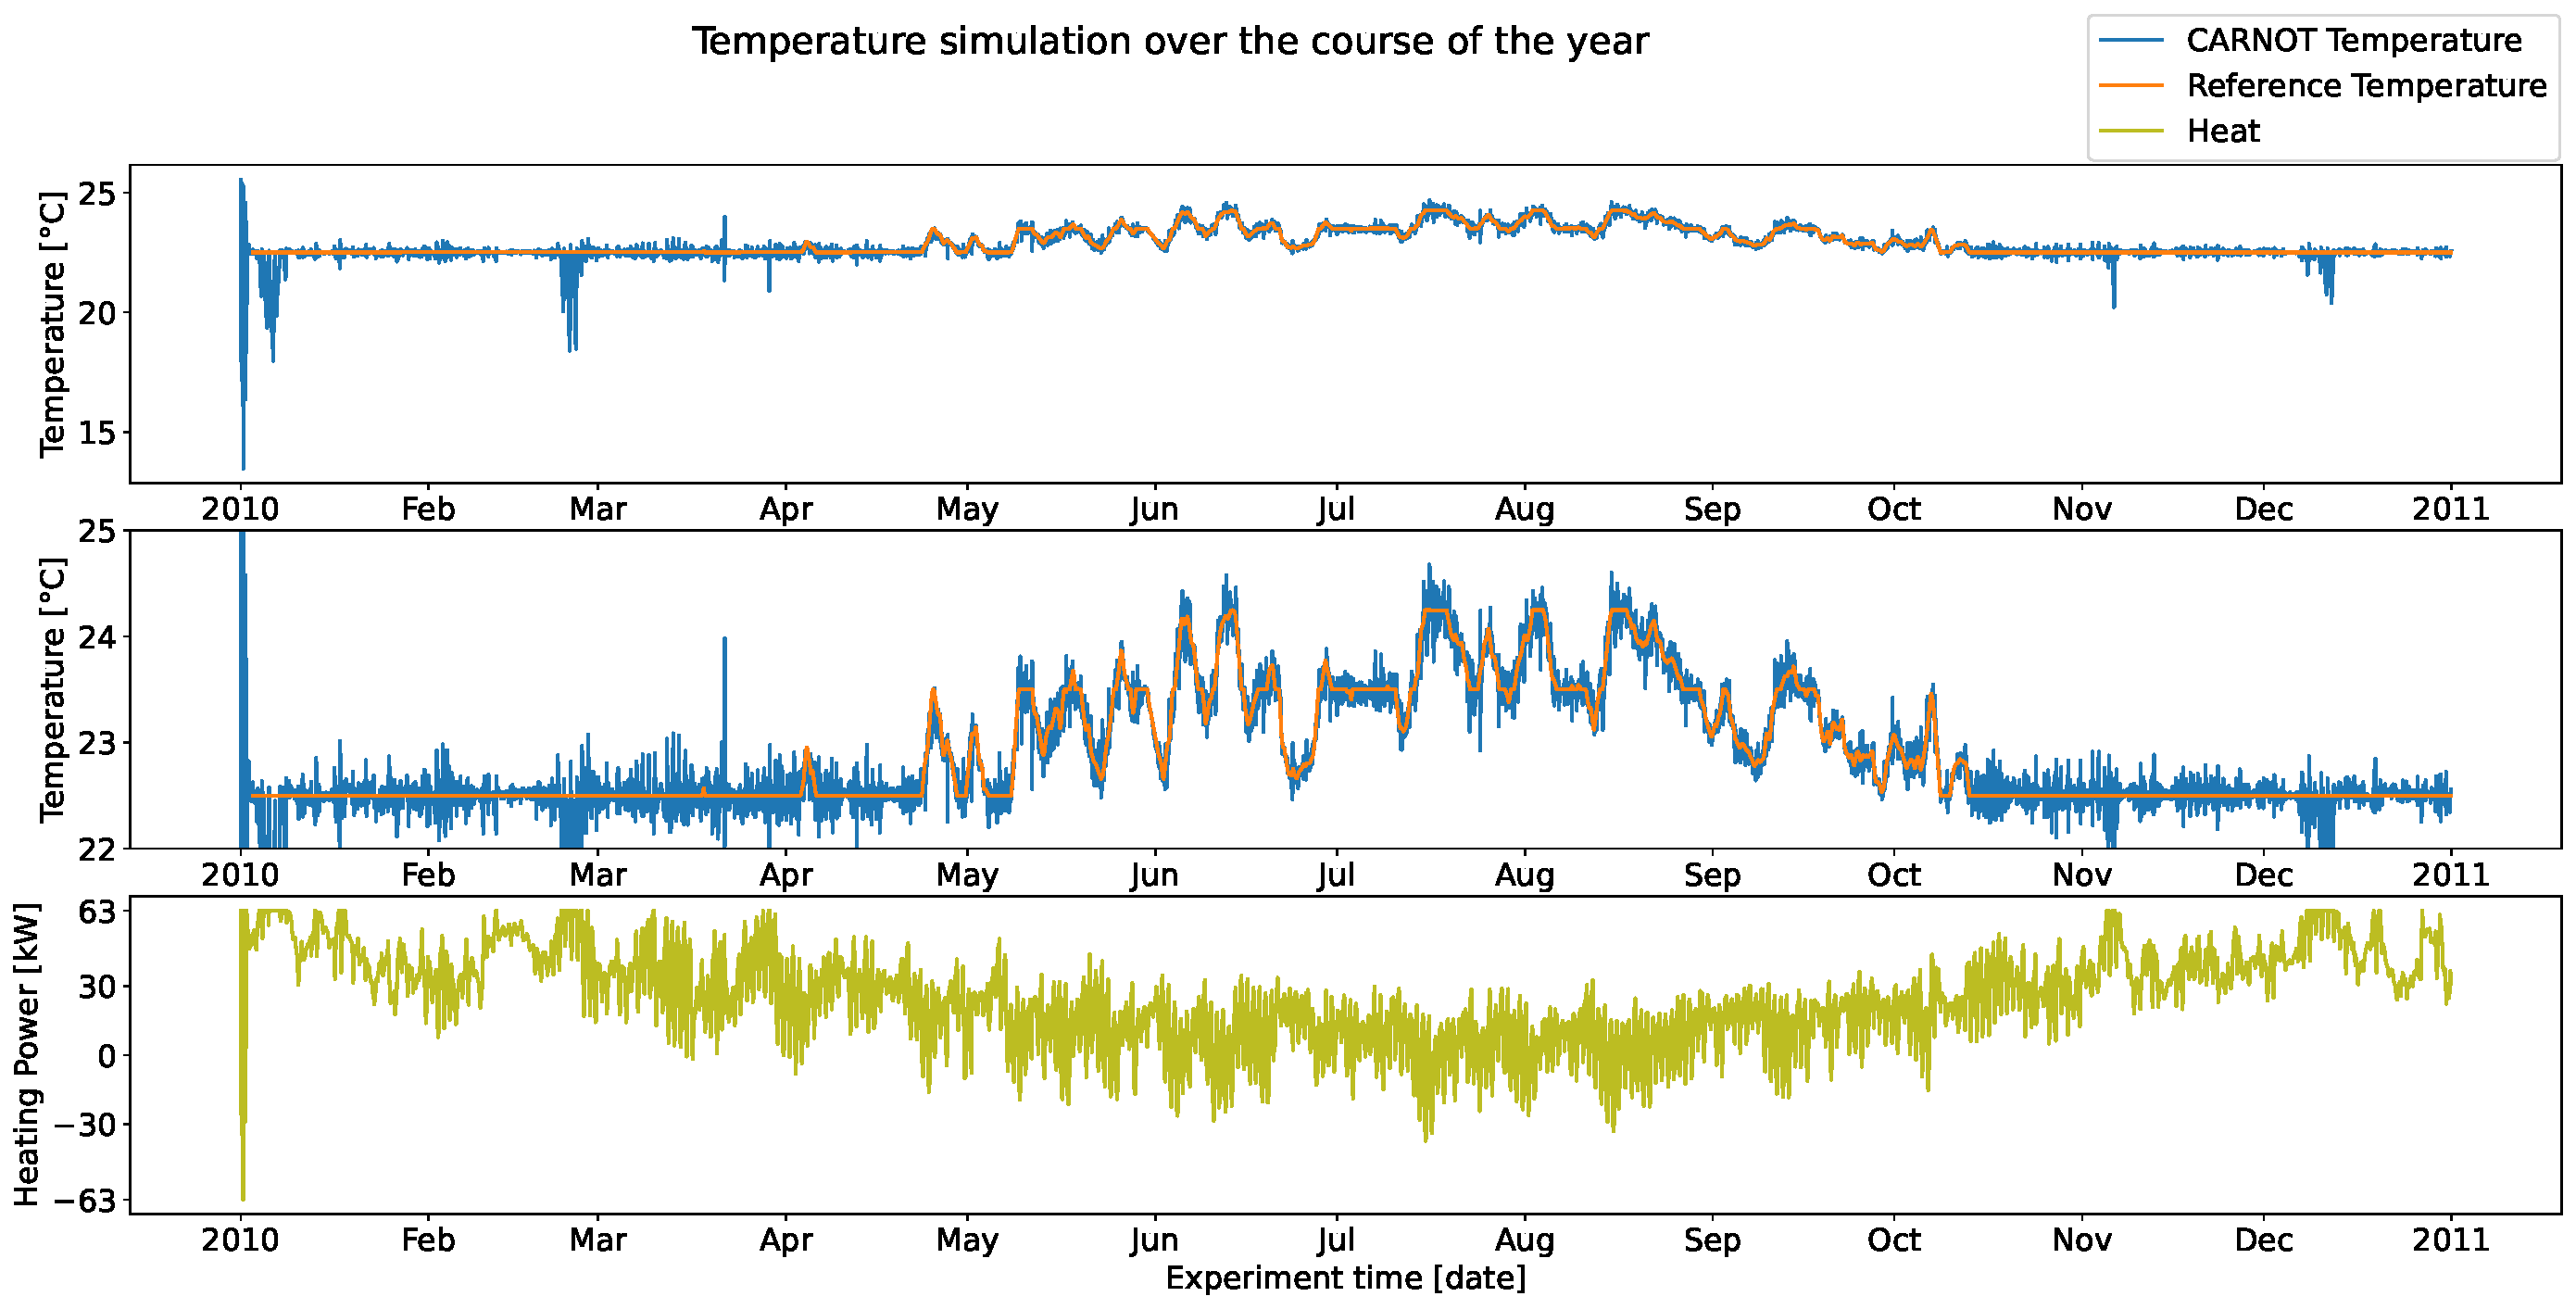
\includegraphics[width =
    \textwidth]{Plots/6_SVGP_96pts_inf_window_12_averageYear_fullyear.pdf}
    \caption{One Day SVGP full year simulation}
    \label{fig:SVGP_96pts_fullyear_simulation}
\end{figure}

\begin{figure}[ht]
    \centering
    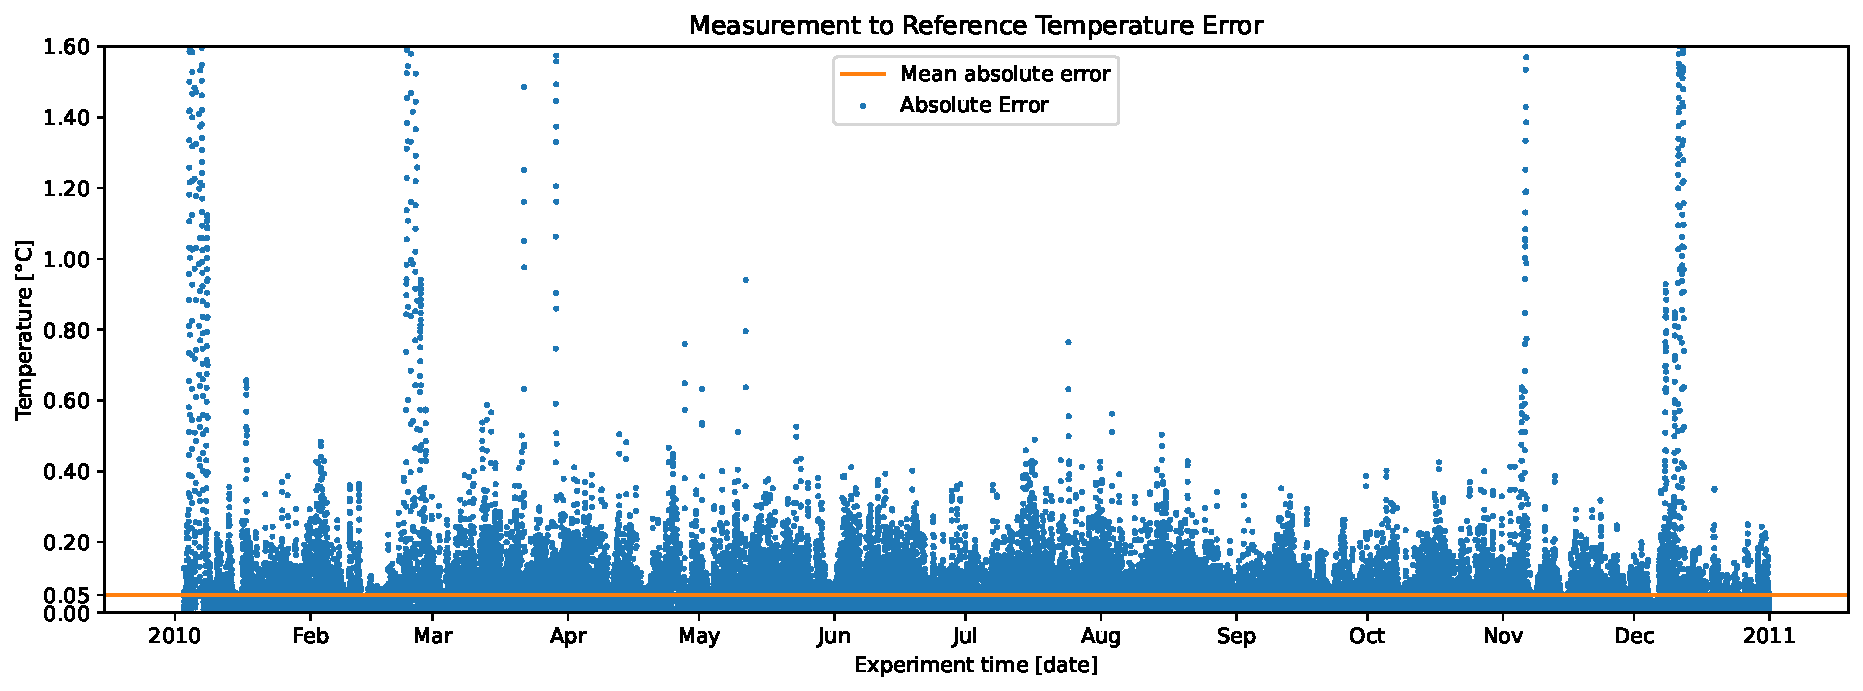
\includegraphics[width =
    \textwidth]{Plots/6_SVGP_96pts_inf_window_12_averageYear_abserr.pdf}
    \caption{One Day SVGP Absolute Error}
    \label{fig:SVGP_96pts_abserr}
\end{figure}

\clearpage

\subsection{SVGP with a five days moving window}\label{sec:svgp_window}

This section presents the result of running a different control scheme. Here, as
was the case for the base \acrshort{svgp} model, it is first trained on 5 days
worth of data, with the difference being that each new model is only identified
using the last five days' worth of data. This should provide an insight on
whether the \acrshort{svgp} model is able to understand model dynamics only
based on closed-loop operation.

\begin{figure}[ht]
    \centering
    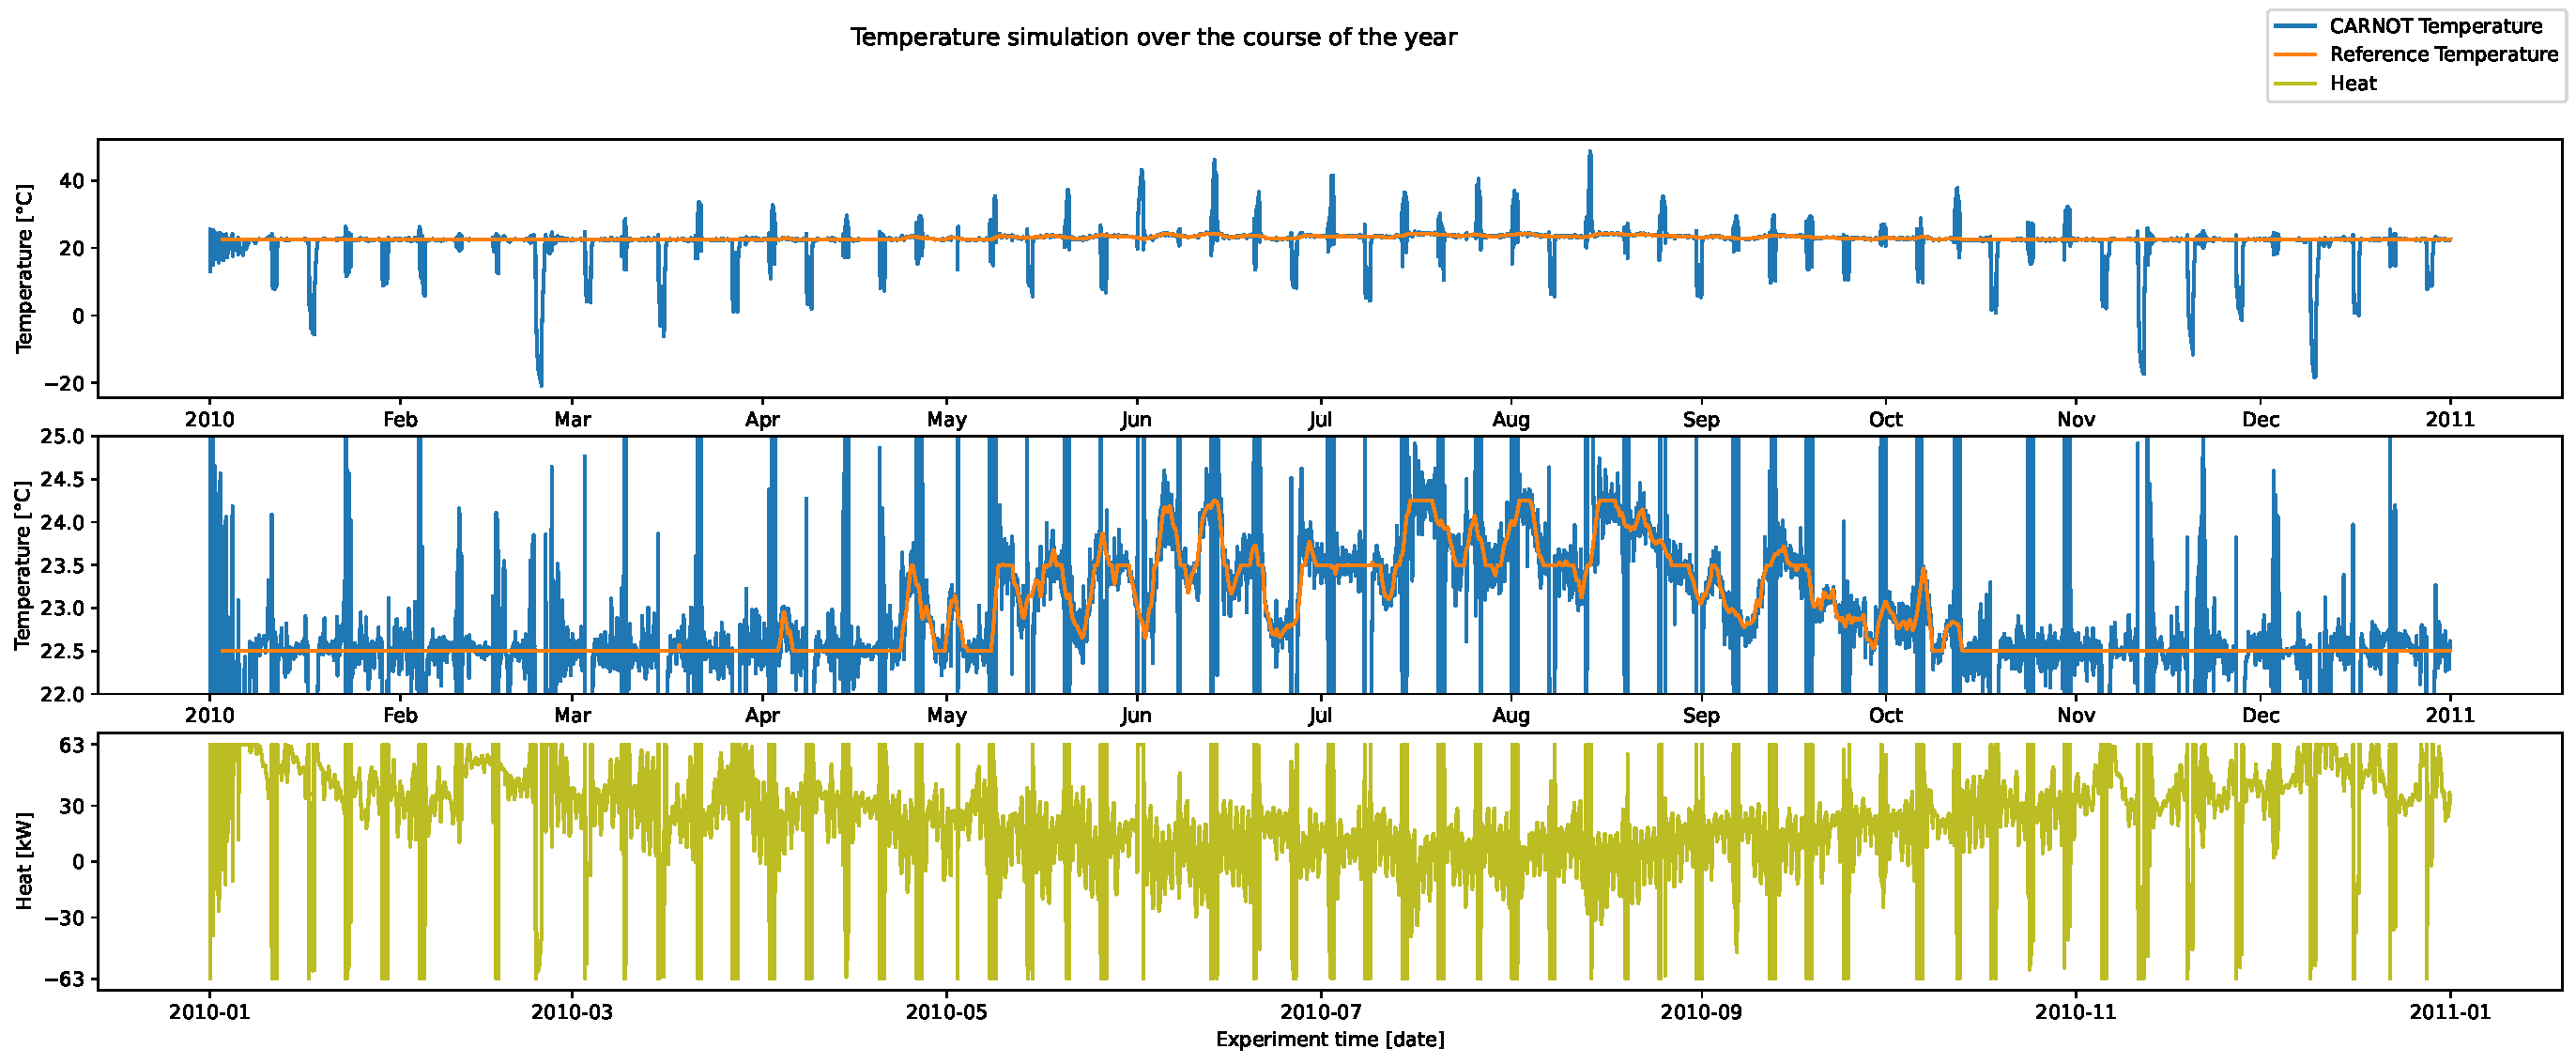
\includegraphics[width =
    \textwidth]{Plots/5_SVGP_480pts_480pts_window_12_averageYear_fullyear.pdf}
    \caption{Windowed SVGP full year simulation}
    \label{fig:SVGP_480window_fullyear_simulation}
\end{figure}

As it can be seen in Figure~\ref{fig:SVGP_480window_fullyear_simulation}, this
model is unable to exhaustively track the reference temperature. In fact, five days
after the identification, the model forgets all the initial data and becomes
unstable. This instability then generates enough excitation of the plant for the
model, to again learn its behaviour. This cycle repeats every five days, when the
controller becomes unstable. In the stable regions, however, the controller is
able to track the reference temperature. 

\clearpage

\subsection{SVGP with Linear Kernel}\label{sec:svgp_linear}

The last model to be investigated is the \acrshort{svgp} with Linear Kernel. As
it was suggested previously, the terms of the originally identified
\acrshort{svgp} model are not very complex, leading to the question whether a
pure linear kernel could suffice to understand the plant's behaviour.

Figure~\ref{fig:SVGP_linear_fullyear_simulation} shows the results of the
full-year simulation. While this controller is still able to track the reference
temperature, it shows a much larger variance in the measured values than the
\acrshort{se} kernel \acrshort{svgp} model. This confirms the previous
suspicions that a pure linear model would not be able to capture the more
nuanced details of the CARNOT model dynamics.

\begin{figure}[ht]
    \centering
    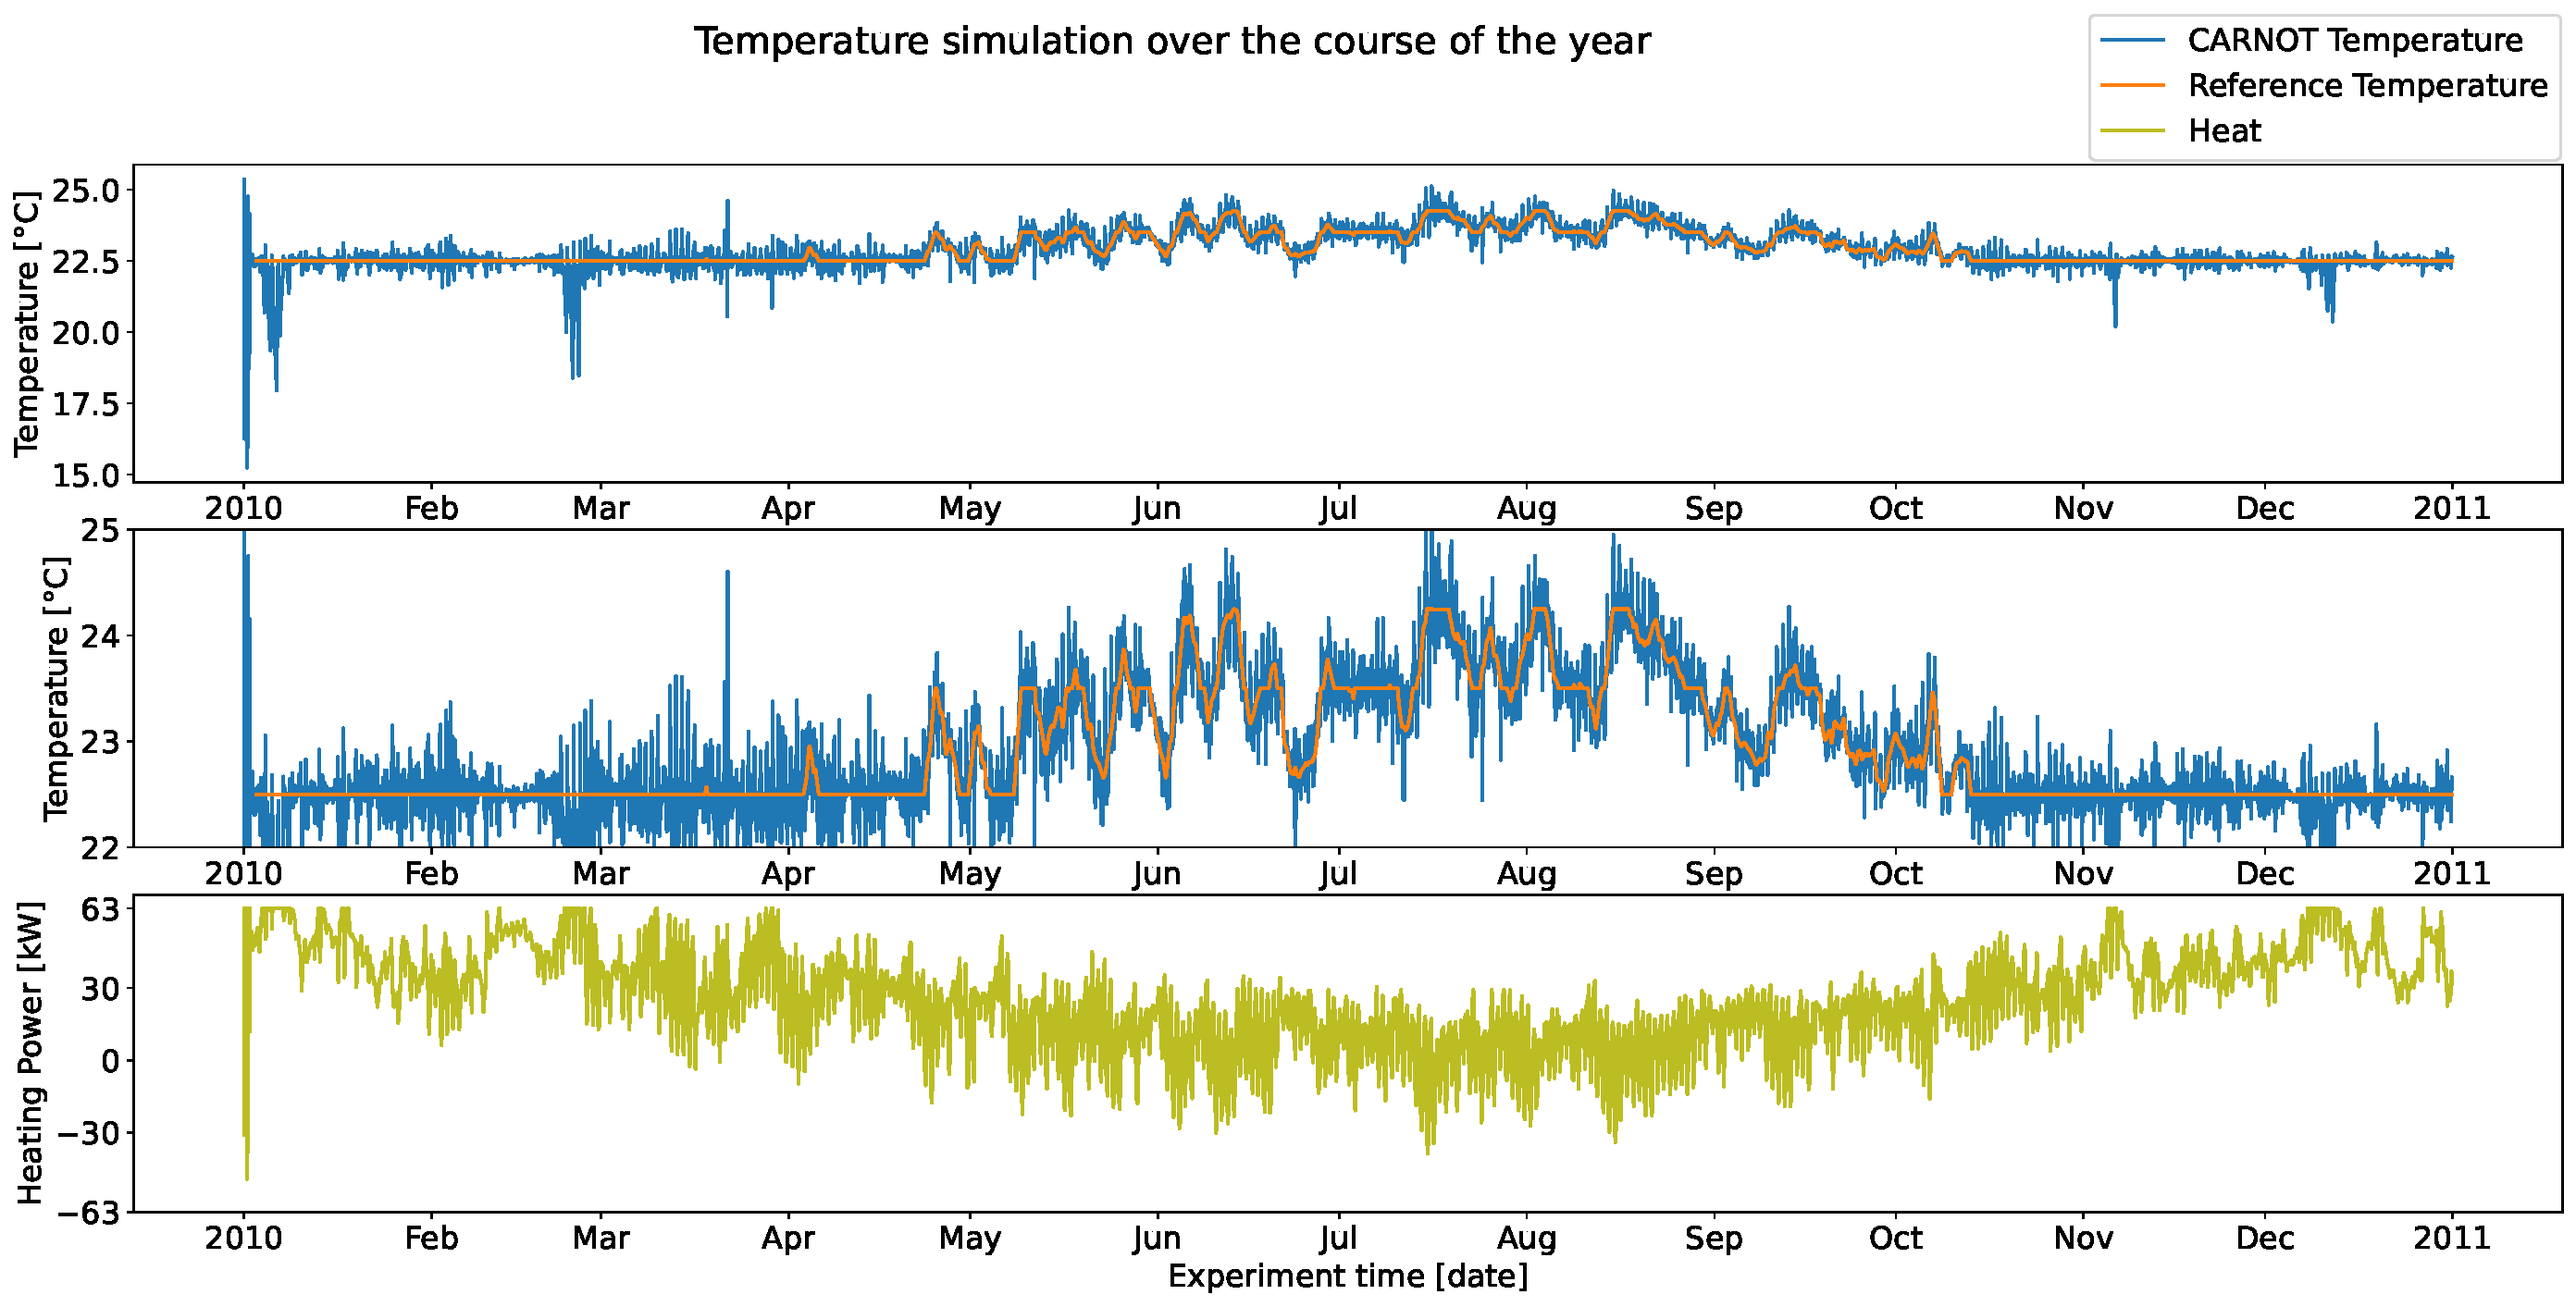
\includegraphics[width =
    \textwidth]{Plots/10_SVGP_480pts_inf_window_12_averageYear_LinearKernel_fullyear.pdf}
    \caption{Linear SVGP full year simulation}
    \label{fig:SVGP_linear_fullyear_simulation}
\end{figure}

\clearpage

\subsection{Comparative analysis}

Presented in Table~\ref{tab:Model_comparations} are the Mean Error, Error
Variance and Mean Absolute Error for the full year simulation for the three
stable \acrshort{svgp} models, as well as the classical \acrshort{gp} model. 

\begin{table}[ht]
%\vspace{-8pt}
\centering
    \begin{tabular}{||c c c c||}
        \hline
        Model & Mean Error [$\degree$C] & Error Variance [$\degree$C] & Mean
        Absolute Error [$\degree$C]\\
        \hline \hline
        GP & 5.08 & 6.88 & 1.330 \\ 
        SVGP (5 days) & -0.06 & 0.25 & 0.055 \\ 
        SVGP (1 day) & -0.04 & 0.24 & 0.050 \\ 
        SVGP (Linear)& -0.03 & 0.29 & 0.093 \\ 
        \hline
    \end{tabular}
\caption{Full-year model performance comparison}
\label{tab:Model_comparations}
\end{table}

The worst performing model, as noted previously, is the \acrshort{gp} model. The
\acrshort{svgp} with Linear Kernel results in a stable model with a mean error
very close to zero, which means no constant bias/ offset. This model has the
highest error variance of all the identified \acrshort{svgp} models, which was
also noted beforehand from qualitative observations. It is therefore possible to
conclude that a Linear Kernel does not suffice for properly modeling the
dynamics of the CARNOT model.

The two \acrshort{svgp} models with \acrlong{se} kernels perform the best. They
have a comparable performance, with very small differences in Mean Absolute
Error and Error variance. This leads to the conclusion that the \acrshort{svgp}
models can be deployed with less explicit identification data, but they will
continue to improve over the course of the year, as the building passes through
different regions of the state space and more data is collected.

However, these results do not discredit the use of \acrlong{gp} for employment
in a multi-seasonal situation. As shown before, given the same amount of data
and ignoring the computational cost, they perform better than the alternative
\acrshort{svgp} models. The bad initial performance could be mitigated by
sampling the identification data at different points in time during multiple
experiments, updating a fixed-size dataset based on the gained information, as
well as more cleverly designing the kernel to include prior information.


\clearpage
